\chapter{European Spallation Source and beam diagnostic devices}
\chaptermark{European Spallation Source and beam diagnostic devices}
\cleardoublepage

\minitoc
\section{Introduction}
\begin{refsection}
  \label{ch2:Introduction}
  The topic of this thesis is the design of non-invasive ionization profile monitors (\acrshort{npm}s) for the \acrshort{ess} proton beam. The European Spallation Source is going to base neutron production on one of the most powerful linear proton accelerators ever built. Beam diagnostic is therefore an essential part of the project, necessary to insure fast tuning of the beam, monitor the beam during neutron production, and provide safety to the machine at any phase of the acceleration operation.

  This chapter gives an overall vision of the \acrshort{ess} project. The different elements of the accelerator will be briefly detailed from the source to the target. In addition, some neutron instruments foreseen at \acrshort{ess} and their applications will be illustrated.

  The second part of the chapter focuses on beam diagnostic devices and their diversity. An exhaustive list of beam diagnostics is not possible and only a few of them are presented here. The chapter concludes with the state of the art of non-invasive profilers based on the ionization of the residual gas.

  \section{European Spallation Source}
  The European Spallation Source is a neutron source facility currently under construction in Lund, Sweden. The objective of \acrshort{ess} is clear: \acrshort{ess} will be the brightest pulsed neutron source in the world and will give to Europe a modern flagship neutron source, as the \acrshort{ill} was.

  \acrshort{ess} can be roughly summarized in 3 parts: a powerful linear accelerator, a large tungsten target and a multitude of neutron scattering instruments. Each of these elements represents a technological breakthrough in their respective fields.

  Fig. \ref{chap3:fig:ESS_pulse} underlines the difference among \acrshort{ess} and existing neutron sources in terms of brightness \footnote{The plot does not have the same scale if power or neutron flux are considered.}.
  \begin{figure}[!ht]
  \begin{center}
    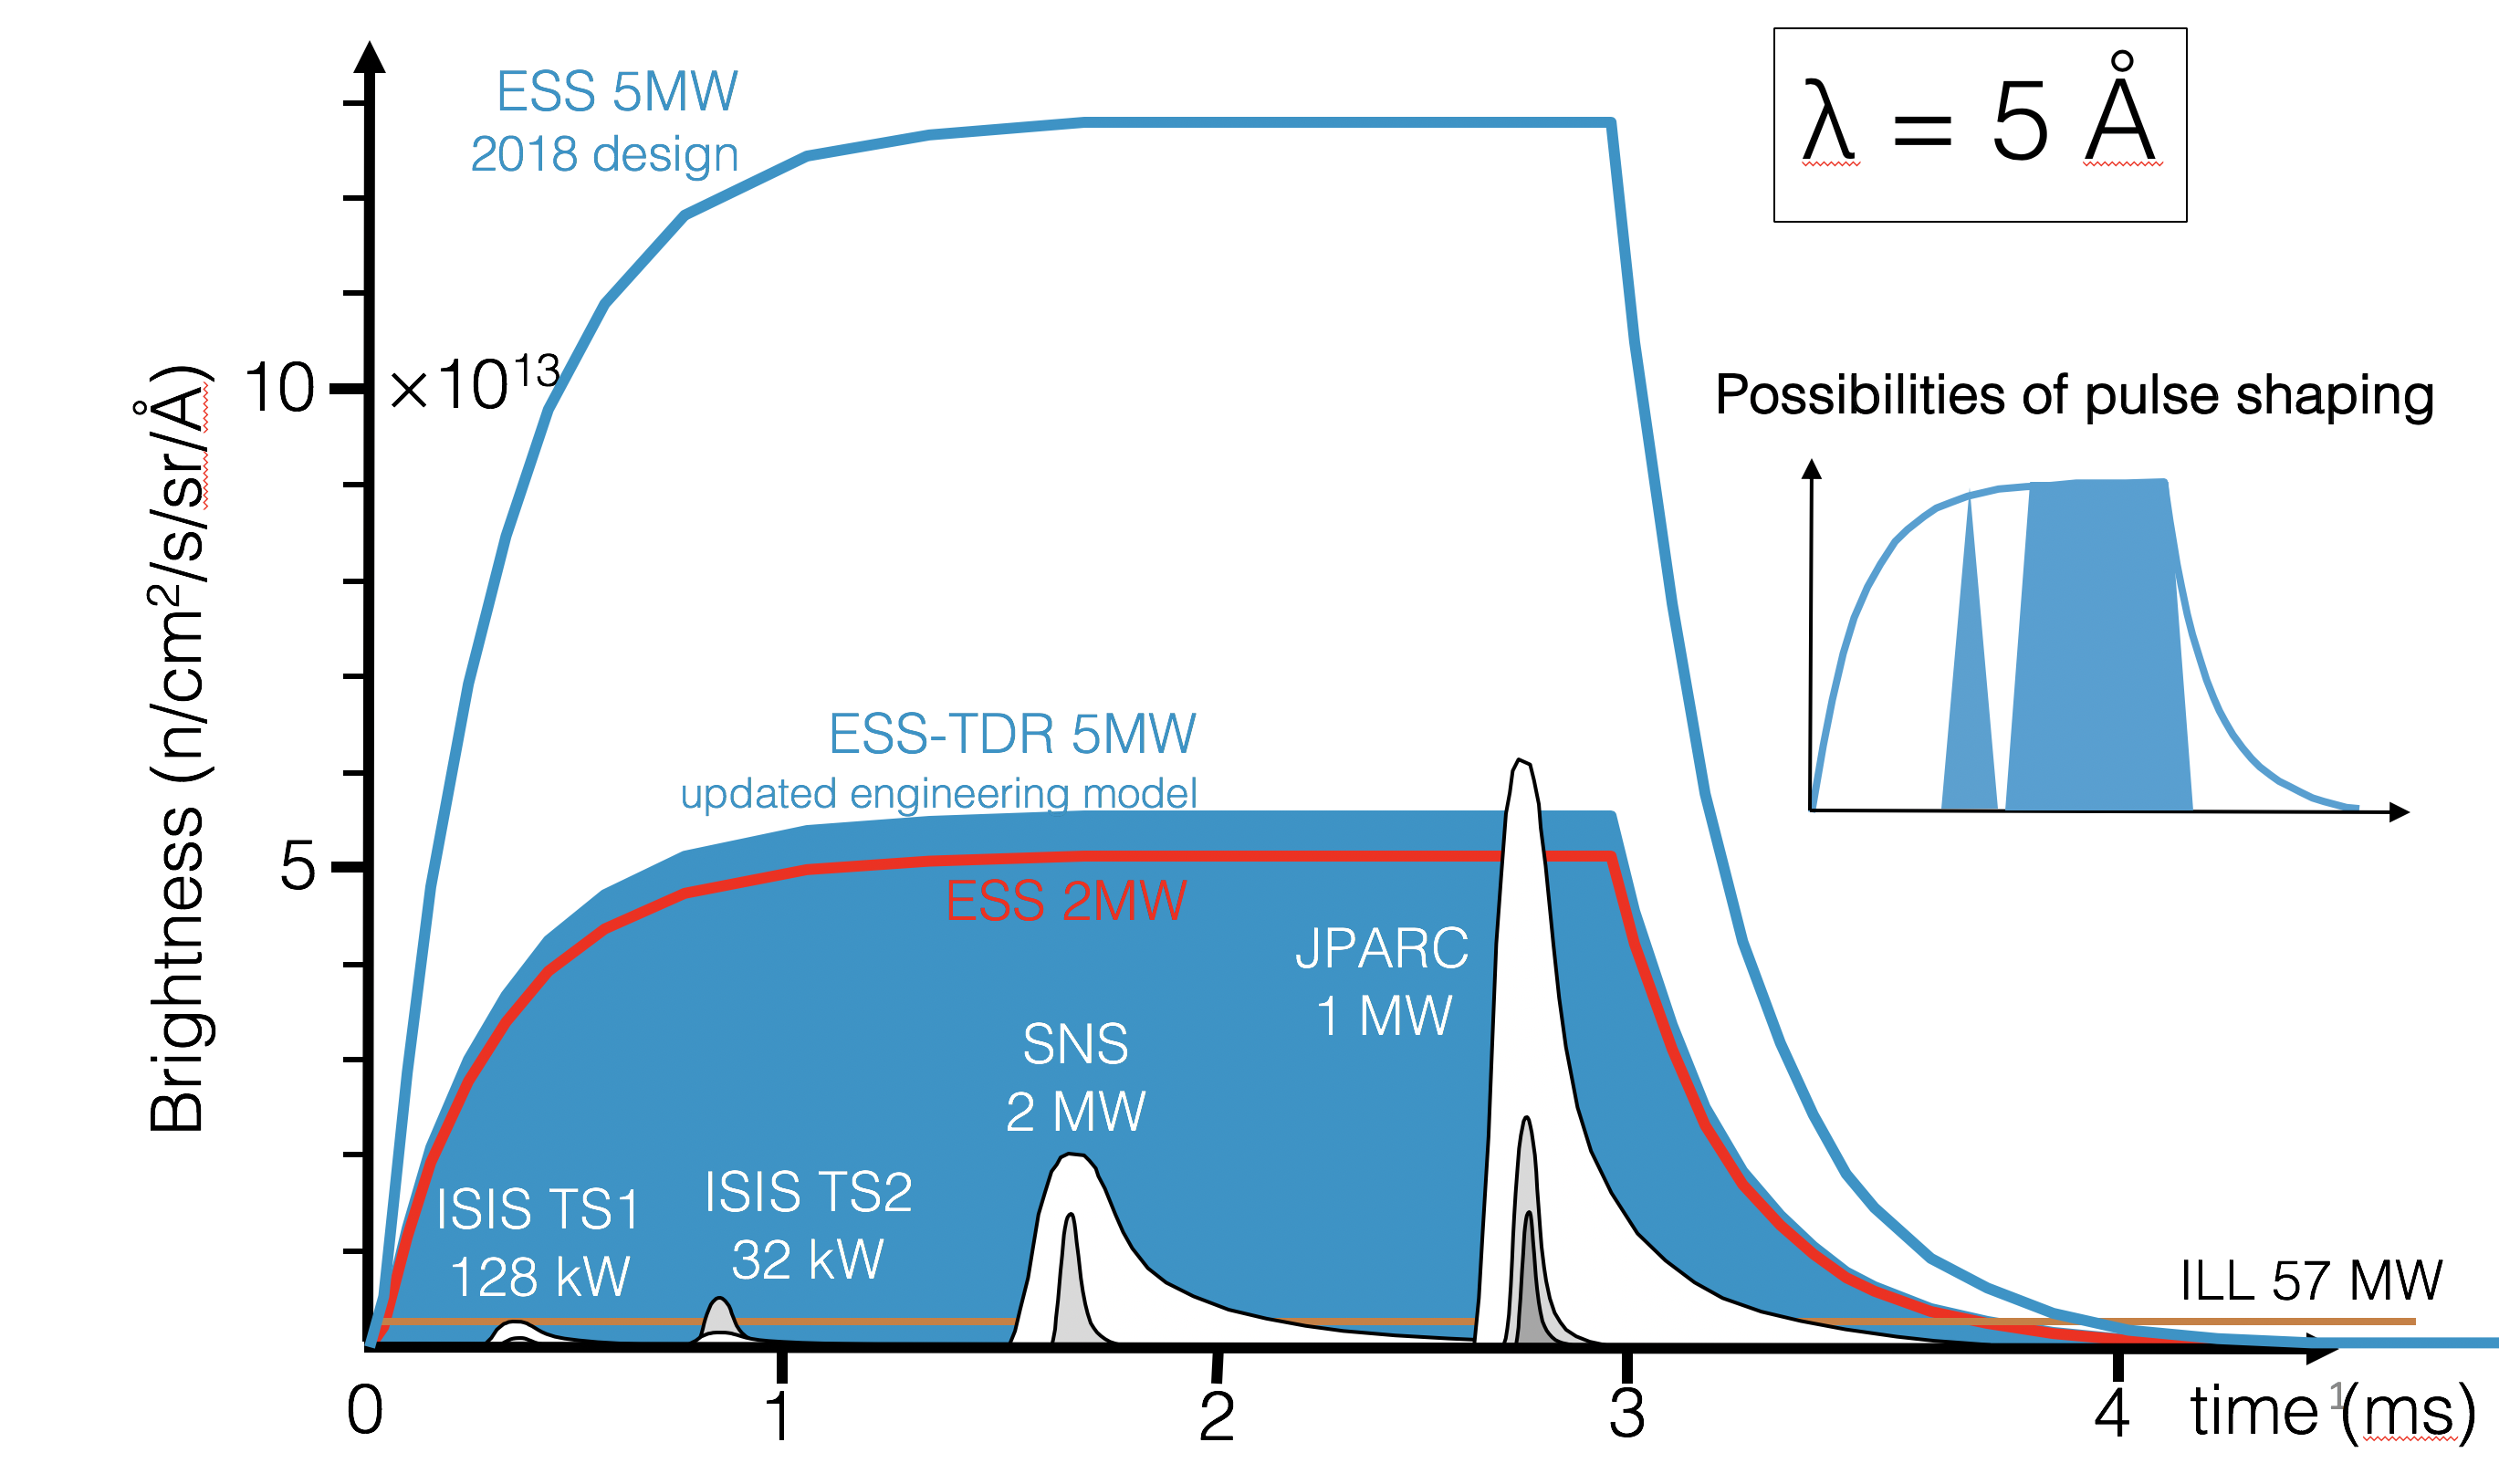
\includegraphics[width=\textwidth]{02_BeamDiag/figures/fig000_ESS_pulse}

  \end{center}
  \caption[ESS neutron source brightness compared to others existing neutron sources]{ESS neutron source brightness compared to others existing neutron sources.}
  \label{chap3:fig:ESS_pulse}
\end{figure}

  
  The specificity of \acrshort{ess} is its linear pulsed high intensity accelerator, which will be one of the most powerful in world. The accelerator is linear from the source to the target and does not require an accumulation ring as \acrshort{sns}. The linac is massively based on superconducting cavities allowing to accelerate long and intense pulses in reasonable dimensions. The total construction cost is estimated at $1843$ million € and the annual operating cost will be about $100$ million € \footnote{The price of electricity can fluctuate significantly, this budget is given as an indication.}.


  The history of \acrshort{ess} is quite complex, its first studies and design dating back to the 1990s. These designs considerably changed over the years, along with the existing technologies.
  % The history of \acrshort{ess} is quite complex, the first studies and design for \acrshort{ess} date back to the 1990s. These designs have changed a lot over the years as well as the existing technologies.
  In the 2000s the project started to become reality, probably due to the beginning of construction of \acrshort{sns} and \acrshort{jsns}.
  In 2009 Lund was chosen to host the future installation. The site is close to the MAX V synchrotron, establishing a scientific hub dedicated to the studies of materials using large instruments.
  The final design of \acrshort{ess} was frozen in 2014 with an energy reduction from $2.5$ to $2\,\mathrm{GeV}$ but an increase of the maximum current to $62.5\,\mathrm{mA}$. The groundbreaking happened in 2014 and in 2017 the accelerator tunnel was completed. The target vault is still under construction. The total progress of the installation is rated at $59\,\mathrm{\%}$. The source and the \acrshort{lebt} were delivered and are functional. The \acrshort{rfq} is expected to be delivered and connected to the \acrshort{lebt} and the \acrshort{mebt} in few weeks. The installation of cryogenic systems supplies is on going. The first protons on target are expected in 2021 whereas the user program will start in 2023.

  \section{ESS activities at CEA/IRFU}

  \acrshort{ess} is a very large project based on an international collaboration of many research Institutes. Today, the collaboration includes more than 140 institutes from 15 different countries with more than 40 European in kind agreements. France is very involved in the \acrshort{ess} project, particularly through two research organizations: the French National Centre for Scientific Research (\acrshort{cnrs}) and the French Alternative Energies and Atomic Energy Commission (\acrshort{cea}).

  \acrshort{cea} is a key player in research, development and innovation in four main areas: defence and security, nuclear and renewable energies, technological research for industry and fundamental research. The Institute for Research on the Fundamental laws of the Universe (\acrshort{irfu}) is one of the institutes attached to the fundamental research division of \acrshort{cea}. \acrshort{irfu} brings together three scientific disciplines: astrophysics, nuclear physics and particle physics. \acrshort{irfu} develops as well the associated technology required by the cutting-edge research.

  %\section{Accelerator basics [En cours de rédaction]}

  \section{ESS accelerator}
  % TODO: ADJ verb ou vrb adj
  The proton linear accelerator (LINAC or linac) of \acrshort{ess} is represented synthetically in Fig. \ref{chap2:fig:ESS_acc}.
  The total length from the source to the target is about $600\,\mathrm{m}$ and $356\,\mathrm{m}$ are dedicated to the acceleration. The first part accelerates the beam up to $90\,\mathrm{MeV}$ by means of conventional room temperature \acrshort{rf} cavities. Then a cold part using superconducting cavities cooled with liquid helium is used to reach the highest energies.

  \begin{figure}[!ht]
	\begin{center}
		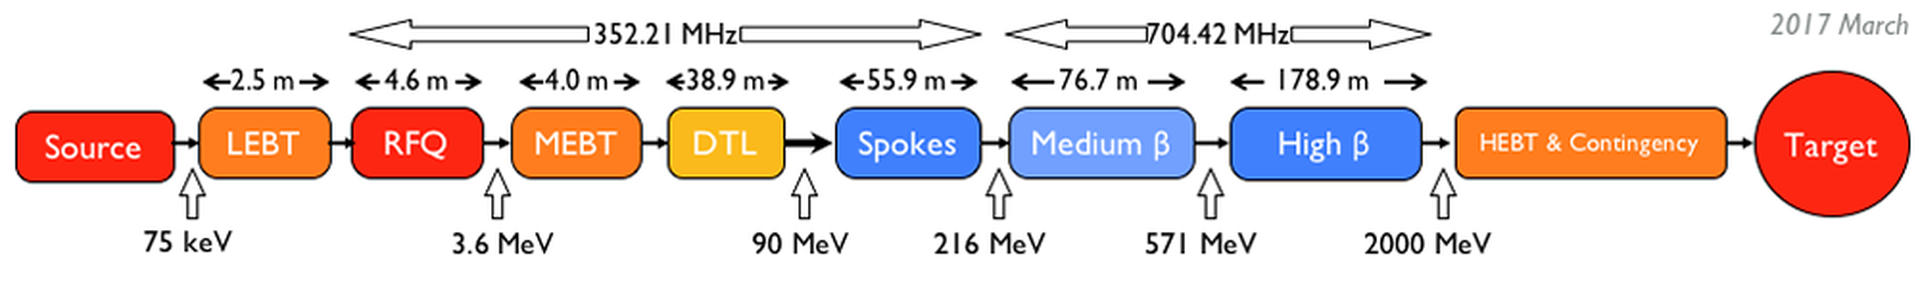
\includegraphics[width=\textwidth]{02_BeamDiag/figures/fig000_ESS_acc}
	\end{center}
	\caption[A simplified representation of the ESS linac]{A simplified representation of the ESS linac. Blue blocks represent superconducting cavities where IPMs will be installed.}
	\label{chap:}
\end{figure}


  Table \ref{chap2:tab:ess_charac} summarizes the most important characteristics of the \acrshort{ess} linac. The particularities of \acrshort{ess} compared to other sources of spallation rely on its very long pulse and its high current. The average beam power is $5\,\mathrm{MW}$ and the peak power is $125\,\mathrm{MW}$, making \acrshort{ess} one of the most powerful proton accelerator in the world.

  \begin{table}[ht]
  \centering
  \caption[ESS nominal conditions]
  {ESS nominal conditions.}
  \label{chap2:ess_charac}
  \begin{tabular}{ll}
    \toprule
    Characteristic    & Value                  \\
    \midrule
    Energy            & $2\,\mathrm{GeV}$      \\
    Current           & $62.5\,\mathrm{mA}$    \\
    Pulse duration    & $2.86\,\mathrm{ms}$    \\
    Power             & $5\,\mathrm{MW}$       \\
    Repetition rate   & $14\,\mathrm{Hz}$      \\
    Duty cycle        & $4\,\mathrm{\%}$       \\
    Radio Frequencies & $352.21\,\mathrm{MHz}$ \\
                      & $704.42\,\mathrm{MHz}$ \\
    \bottomrule
  \end{tabular}
\end{table}

  In the next sections the role of each of the accelerator blocks is described in few words and detailed reviews of the \acrshort{ess} project are available in the following \cite{Peggs2013, Garoby2017}.

  \subsection{Ion source and Low Energy Beam Transport}
  The source is the first stage of any accelerator: it creates and extracts the plasma. An \acrfull{ecr} source is a type of source particularly suitable for the production of plasma of mono specie at high intensity \cite{nicke2012}. An \acrshort{ecr} source is based on the superposition of a magnetic field and a \acrshort{rf} wave. In a magnetic field the electrons orbit around the magnetic field lines with a frequency defined by:
  \begin{equation}
    \omega_{e} = \frac{eB}{m_{e}}
  \end{equation}
  By injecting a powerful \acrshort{rf} wave of the same frequency, the electrons will enter in resonance and reach sufficient energy to ionize the medium and create a plasma. In an \acrshort{ecr} source the plasma is confined by the magnetic field. Then, a series of electrodes placed at very high potential extract the plasma from the confinement chamber. At the source output, the beam has an energy close to $100\,\mathrm{keV}$. For instance the \acrshort{ess} source accelerates
  protons to $75\,\mathrm{keV}$.
  \begin{figure}[!ht]
	\begin{center}
		\includegraphics[width=\textwidth]{example-image-a}
	\end{center}
	\caption[]{}
	\label{chap:}
\end{figure}


  At low energies the plasma is strongly affected by space charge effects and is therefore very divergent. The \acrfull{lebt} contains the space charge by using solenoids, and optimizes the injection of the plasma into the first accelerating cavity (\acrshort{rfq}).
  Fig. \ref{chap2:fig:LEBT_ESS} outlines the source and the \acrshort{lebt} of \acrshort{ess}. An iris allows to finely adjust the beam current and a Faraday cage is able to measure the current. This line also contains diagnostics that check the quality of the beam before the injection into the \acrshort{rfq}: the Alison scanners to measure the emittance of the beam, the Doppler Shift unit to measure the transported fraction species ($H^{+}$, $H_{2}^{+}$, $H_{3}^{+}$), and \acrshort{npm}s to measure the beam position and beam size. These diagnostics are critical to establish the matching condition to enter the \acrshort{rfq}.

  The \acrshort{infn} Catania was in charge of the design and production of the source and the \acrshort{lebt}. \acrshort{cea}/\acrshort{irfu} was involved in two diagnostics: a Doppler Shift Unit \cite{Thomas:IPAC2017-MOPVA037} and an Allison \cite{Tuske:IPAC2017-MOPAB023}. The source was delivered at \acrshort{ess} and commissioned in 2018.

  \subsection{Radio Frequency Quadrupole}
  The principle of the \acrfull{rfq} was imagined in the 1970s in Russia by I. M. Kapchinskiy and V. Tepliakov. The method quickly became popular and essential in very intense accelerators since it is still the most efficient method for bunching and accelerating particles at low energies.

  At these energies, the space charge is so high that the beam divergence is enormous and must be compensated. A \acrshort{rfq} behaves as a sequence of focusing and defocusing elements that can contain the space charge. \acrshort{rf} waves are propagated on four poles, usually vanes (Fig. \ref{chap2:fig:RFQ_c}) or rods, with opposite amplitude between each pole (Fig. \ref{chap2:fig:RFQ_a}). The \acrshort{rf} variation allows to successively focus in one direction (and defocus in the other direction). A mechanical modulation of the vanes introduces a longitudinal electric field that will accelerate the particles (Fig. \ref{chap2:fig:RFQ_b}). The roles of the \acrshort{rfq} are:
  \begin{itemize}
    \item containing and focusing the beam;
    \item structuring the beam into small bunches;
    \item accelerating the particles.
  \end{itemize}

  \begin{figure}[!ht]
  \centering
  \begin{subfigure}[t]{0.3\textwidth}
    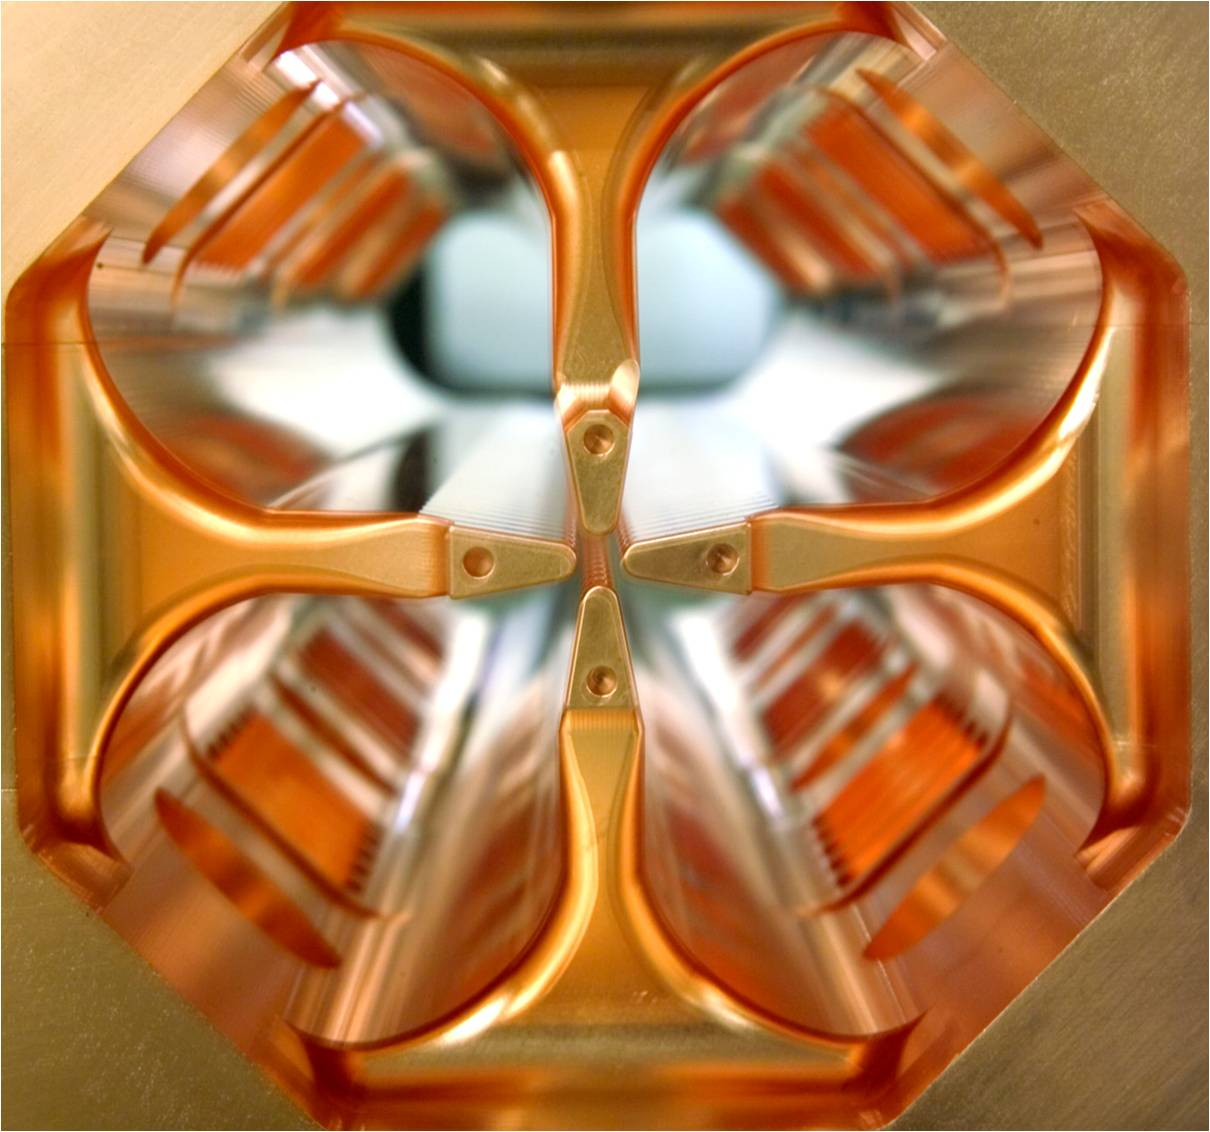
\includegraphics[width=\textwidth]{02_BeamDiag/figures/fig000_RFQ_c}
    \caption[The four copper vanes of a RFQ]{The four copper vanes (poles) of a RFQ.}
    \label{chap2:fig:RFQ_c}
  \end{subfigure}
  ~
  \begin{subfigure}[t]{.3\textwidth}
    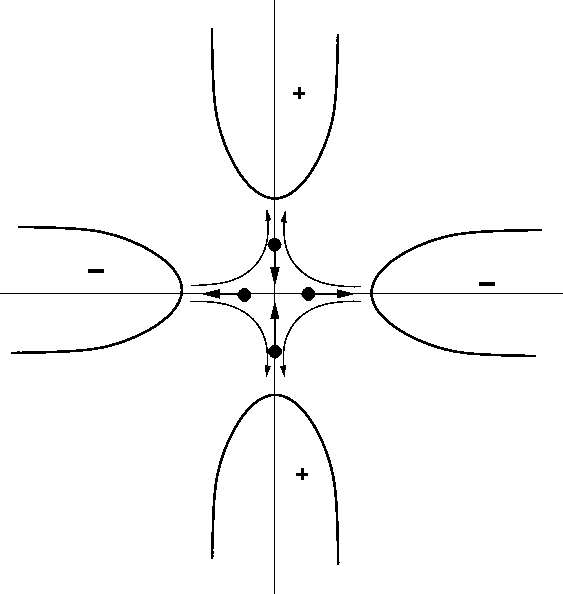
\includegraphics[width=\textwidth]{02_BeamDiag/figures/fig000_RFQ_a}
    \caption{Cut view of the transverse field.}
    \label{chap2:fig:RFQ_a}
  \end{subfigure}
  ~
  \begin{subfigure}[t]{0.3\textwidth}
    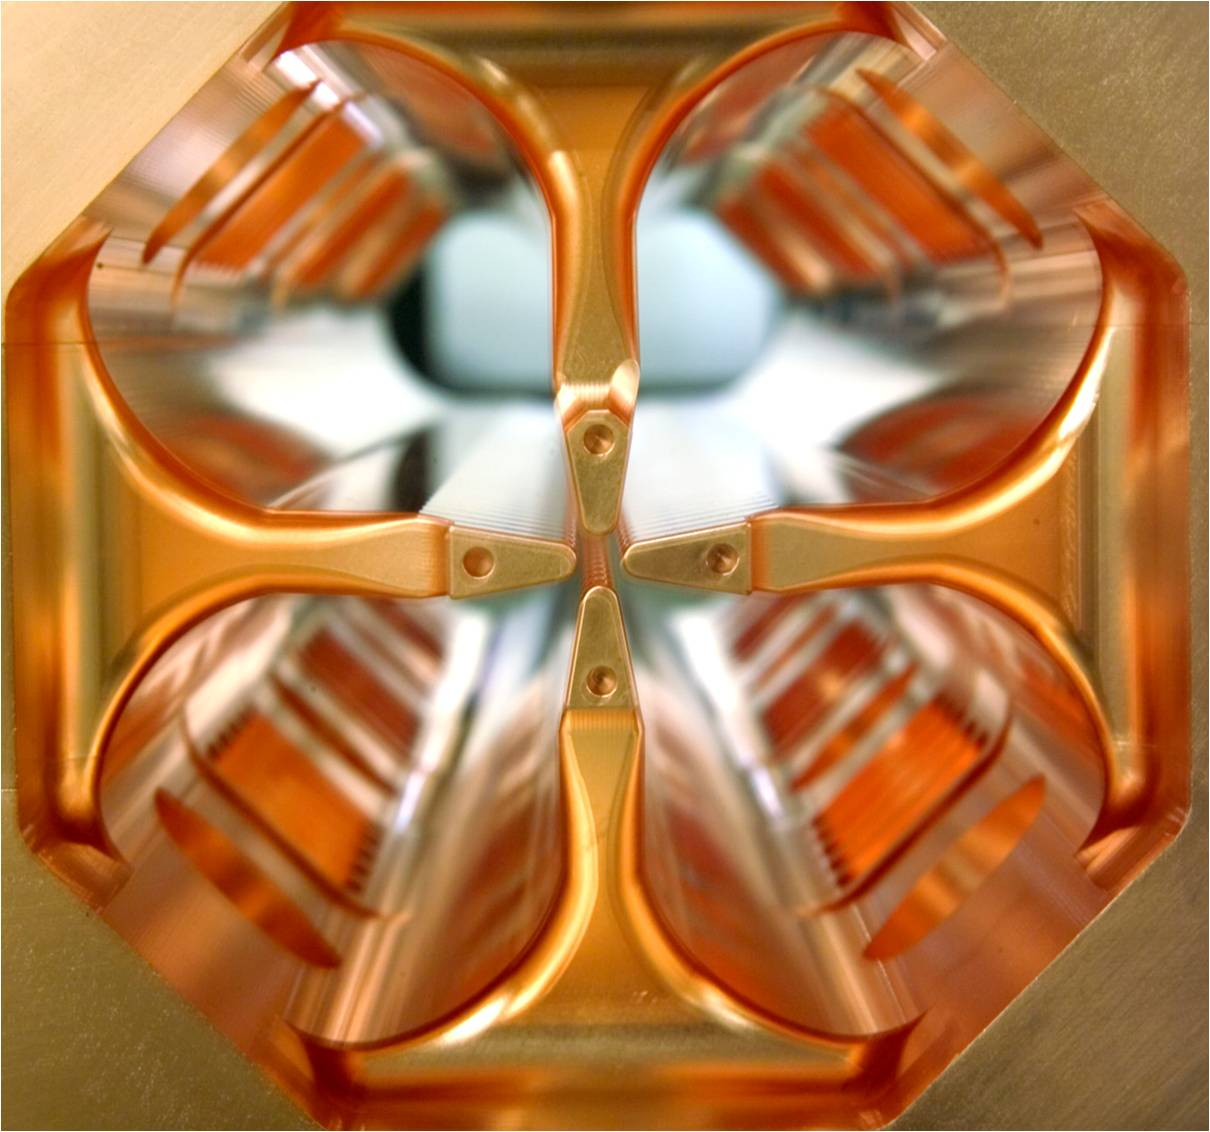
\includegraphics[width=\textwidth]{02_BeamDiag/figures/fig000_RFQ_b}
    \caption[Longitudinal modulation leading to an accelerating field]{Longitudinal modulation leading to an accelerating field \cite{Lombardi:1005049}.}
    \label{chap2:fig:RFQ_b}
  \end{subfigure}

  \caption[An RFQ structure bunches, focuses and accelerates charged particles by means of four poles that modulate the RF wave.]{An RFQ structure bunches, focuses and accelerates charged particles by means of four poles that modulate the RF wave.}
  \label{chap2:fig:RFQ}
\end{figure}


  The simulations of such device are complicated and require specific codes to compute the propagation of the \acrshort{rf} waves and the transport of particles inside the \acrshort{rfq} \cite{Duperrier2000}. In addition, the conception of this type of cavities is extremely technical: for instance the tolerance on the mechanical structures of the vanes is in the order of micrometers whereas the whole \acrshort{rfq} structure often exceeds meters.

  The \acrshort{cea}/\acrshort{irfu} is in charge of the construction of the \acrshort{ess} \acrshort{rfq} \cite{ChirpazIPAC2016} which accelerates the proton beam at the source exit from $75\,\mathrm{keV}$ up to $3.6\,\mathrm{MeV}$ and bunches them with a $352.21\,\mathrm{MHz}$ frequency.

  \subsection{Medium Energy Beam Transport and Drift Tube Linac}
  The \acrfull{mebt} is located just downstream of the \acrshort{rfq} and contains beam optical elements, buncher cavities and beam diagnostics allowing beam characterization and correction. Fig. \ref{chap2:fig:MEBT} shows a block view of the \acrshort{mebt} and its different elements. Most diagnostics will be presented later in the chapter and a table of abbreviations is available at the end of the thesis. The \acrshort{mebt} has been developed by the ESS-Bilbao team.
  \begin{figure}[!ht]
	\begin{center}
		\includegraphics[width=\textwidth]{example-image-a}
	\end{center}
	\caption[]{}
	\label{chap:}
\end{figure}


  \begin{figure}[!ht]
	\begin{center}
		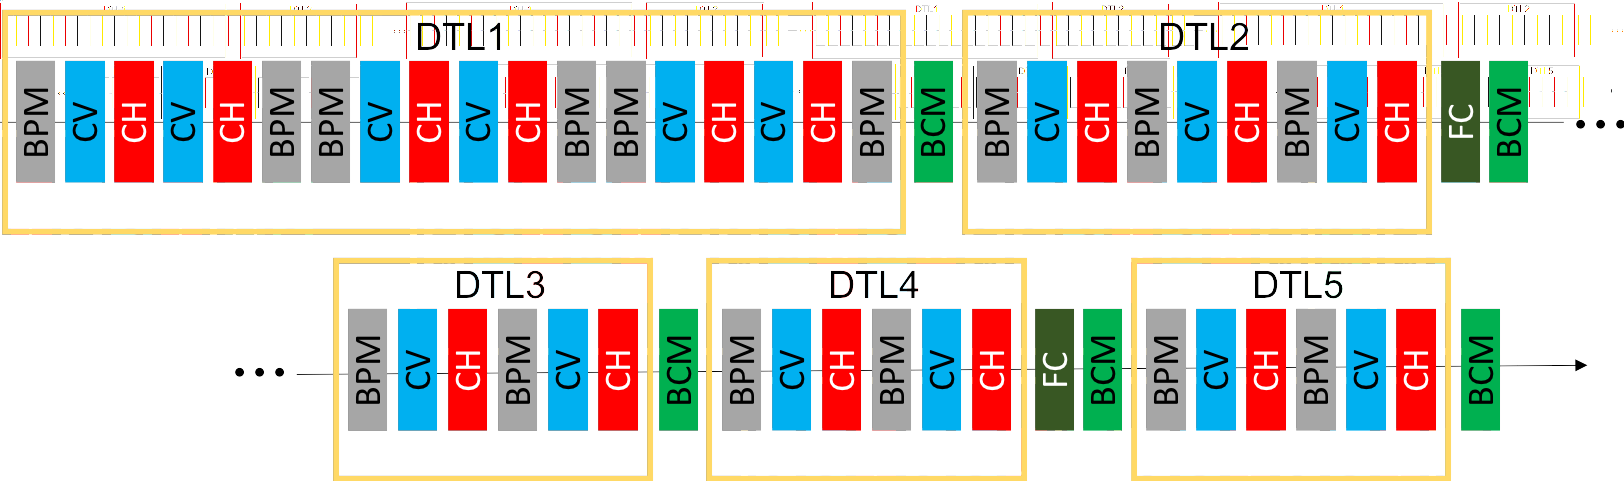
\includegraphics[width=\textwidth]{02_BeamDiag/figures/fig000_DTL}
	\end{center}
	\caption[Building blocks of the MEBT]{Building blocks of the MEBT.}
	\label{chap2:fig:DTL}
\end{figure}
  The \acrshort{mebt} prepares the beam for the injection in the \acrfull{dtl}\footnote{Sometimes, the structure is referred as Alvarez Drift Tube Linac.}.
  A \acrshort{dtl} cavity is a cylindrical standing waves resonant structure. It uses coaxial cylinders (drift tubes) fixed at one end of support tubes. The acceleration occurs in the gaps between two cylinders. The cylinders are also designed to shield the field for particles during the deceleration phase. The length of these drift tubes increases along the structure since it is related to the particle velocity. Permanent quadrupole magnets are encapsulated within the coaxial cylinders allowing a radial focusing of the beam.

  At \acrshort{ess}, the \acrshort{dtl}s are designed to accelerate the beam from $3.62\,\mathrm{MeV}$ to $90\,\mathrm{MeV}$. The \acrshort{ess} \acrshort{dtl}s have similar design to the Linac4 \acrshort{dtl}s. The \acrshort{dtl}s are separated in five \acrshort{dtl} tanks containing between 61 to 23 drift tubes. Fig. \ref{chap2:fig:DTL} presents some pictures of the \acrshort{ess} \acrshort{dtl}s.


  \subsection{Superconducting cavities}
  The \acrshort{dtl}s are not optimized beyond 100 MeV because the length of the drift tubes becomes too long. Two solutions can be considered: increasing the accelerating field or increasing the radio frequency. However, both solutions are technically difficult to implement for long pulsed beams. Indeed, losses in the cavities become very high leading to inefficient acceleration and heating the cavities. The use of superconducting \acrshort{rf} cavities overcomes these issues. These superconducting cavities act as perfect conductors when the transition temperature of the superconductor is reached: $9.2\,\mathrm{K}$ for niobium.

  The cooling of these cavities is done by a liquid helium system working at $4.13\,\mathrm{K}$, enclosed in a tank with thermal shielding, including circuitry for the cooling of cavities, couplers, magnets... The assembly process of such cryomodules must be done in clean conditions and in a particle free environment (ISO-5 cleanrooms). A defect on surfaces or contaminations may lead to a loss of the superconductivity capability locally, increasing the \acrshort{rf} losses and temperature in this area: a quench.
  In addition, superconducting cavities are very affected by field emissions.

  Our devices will be installed between two cryomodules, and therefore must be compliant with the constraints imposed by the use of superconducting cavities at \acrshort{ess}. The \acrshort{cea}/\acrshort{irfu} is responsible for the design and integration of medium and high beta cryomodules. Fig. \ref{chap2:fig:ESS_cryo} pictures one elliptical cryomodule.

  \begin{figure}[!ht]
	\begin{center}
		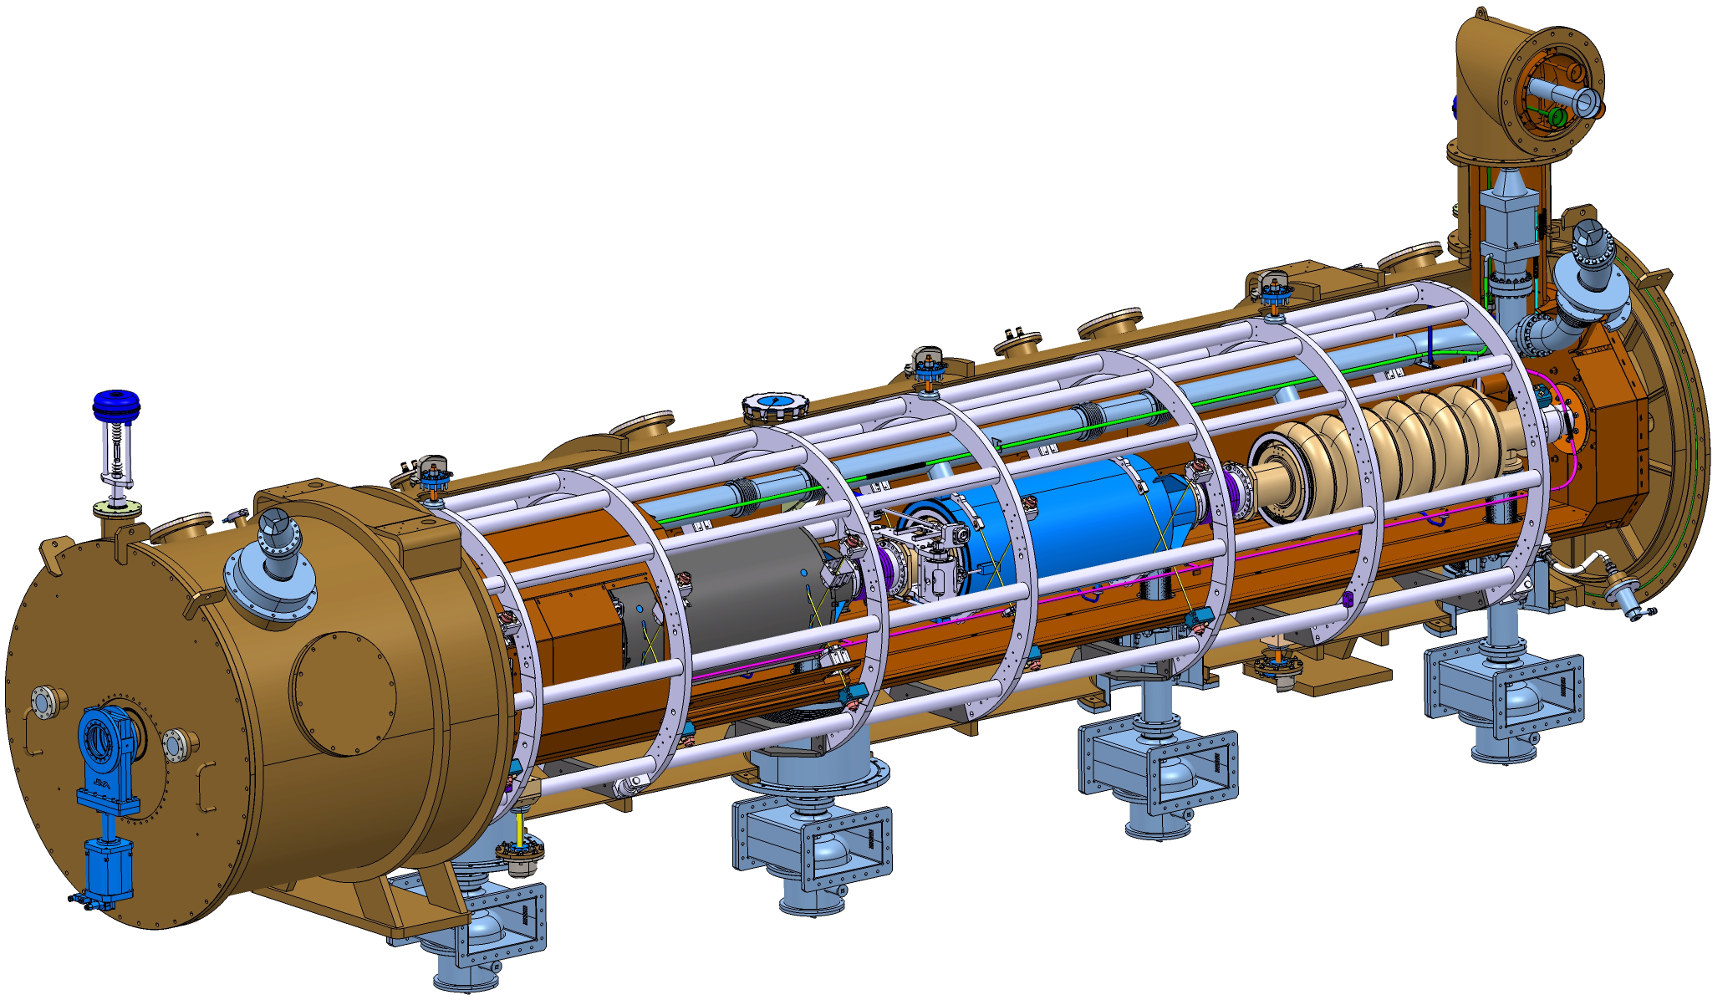
\includegraphics[width=\textwidth]{02_BeamDiag/figures/fig000_cryo_a2}
	\end{center}
	\caption[ESS medium beta elliptical cavities cryomodule]{ESS medium beta elliptical cavities cryomodule.}
	\label{chap2:fig:ESS_cryo}
\end{figure}


  \section{Transport lines and target}
  The protons are then transported in a \acrfull{hebt} line to the target \footnote{The target is at a different ground level compare to the accelerator.}. A beam dump will be also used during the commissioning phase of the accelerator. The \acrshort{hebt} contains beam diagnostics and beam optic elements that prepare the beam for impacting on the target.

  The \acrshort{ess} target should be designed to optimize the neutron yield from the spallation reaction and to sustain the $5\,\mathrm{MW}$ beam power. Two technologies are commonly used for spallation targets:
  \begin{itemize}
    \item Solid targets with active cooling (ISIS, SINQ).
    \item Liquid targets with liquid recirculation (\acrshort{sns}, \acrshort{jsns}).
  \end{itemize}
  The solution chosen by \acrshort{ess} is a solid target wheel of diameter of $2.3\,\mathrm{m}$. The wheel will rotate at $23.33\,\mathrm{rpm}$. The wheel is composed of more than $7000$ small tungsten bricks giving a total weight of around 5 tons. The bricks are cooled with liquid helium. The design of the target requires extensive thermal and mechanical studies. All these activities and the manufacturing of the target, as well as many other systems around the target, are under the responsibility of ESS-Bilbao.

  The neutron flux is maximized by means of moderator-reflectors and thermalized by different water and liquid $H_{2}$ moderators. The neutron brightness is more or less uniform over the 42 neutron ports around the target. The target moderators and all other systems (engine, cooling etc.) are contained in a shielded structure: the monolith. The monolith is visible in Fig. \ref{chap2:fig:target}.

  \begin{figure}[!ht]
	\begin{center}
		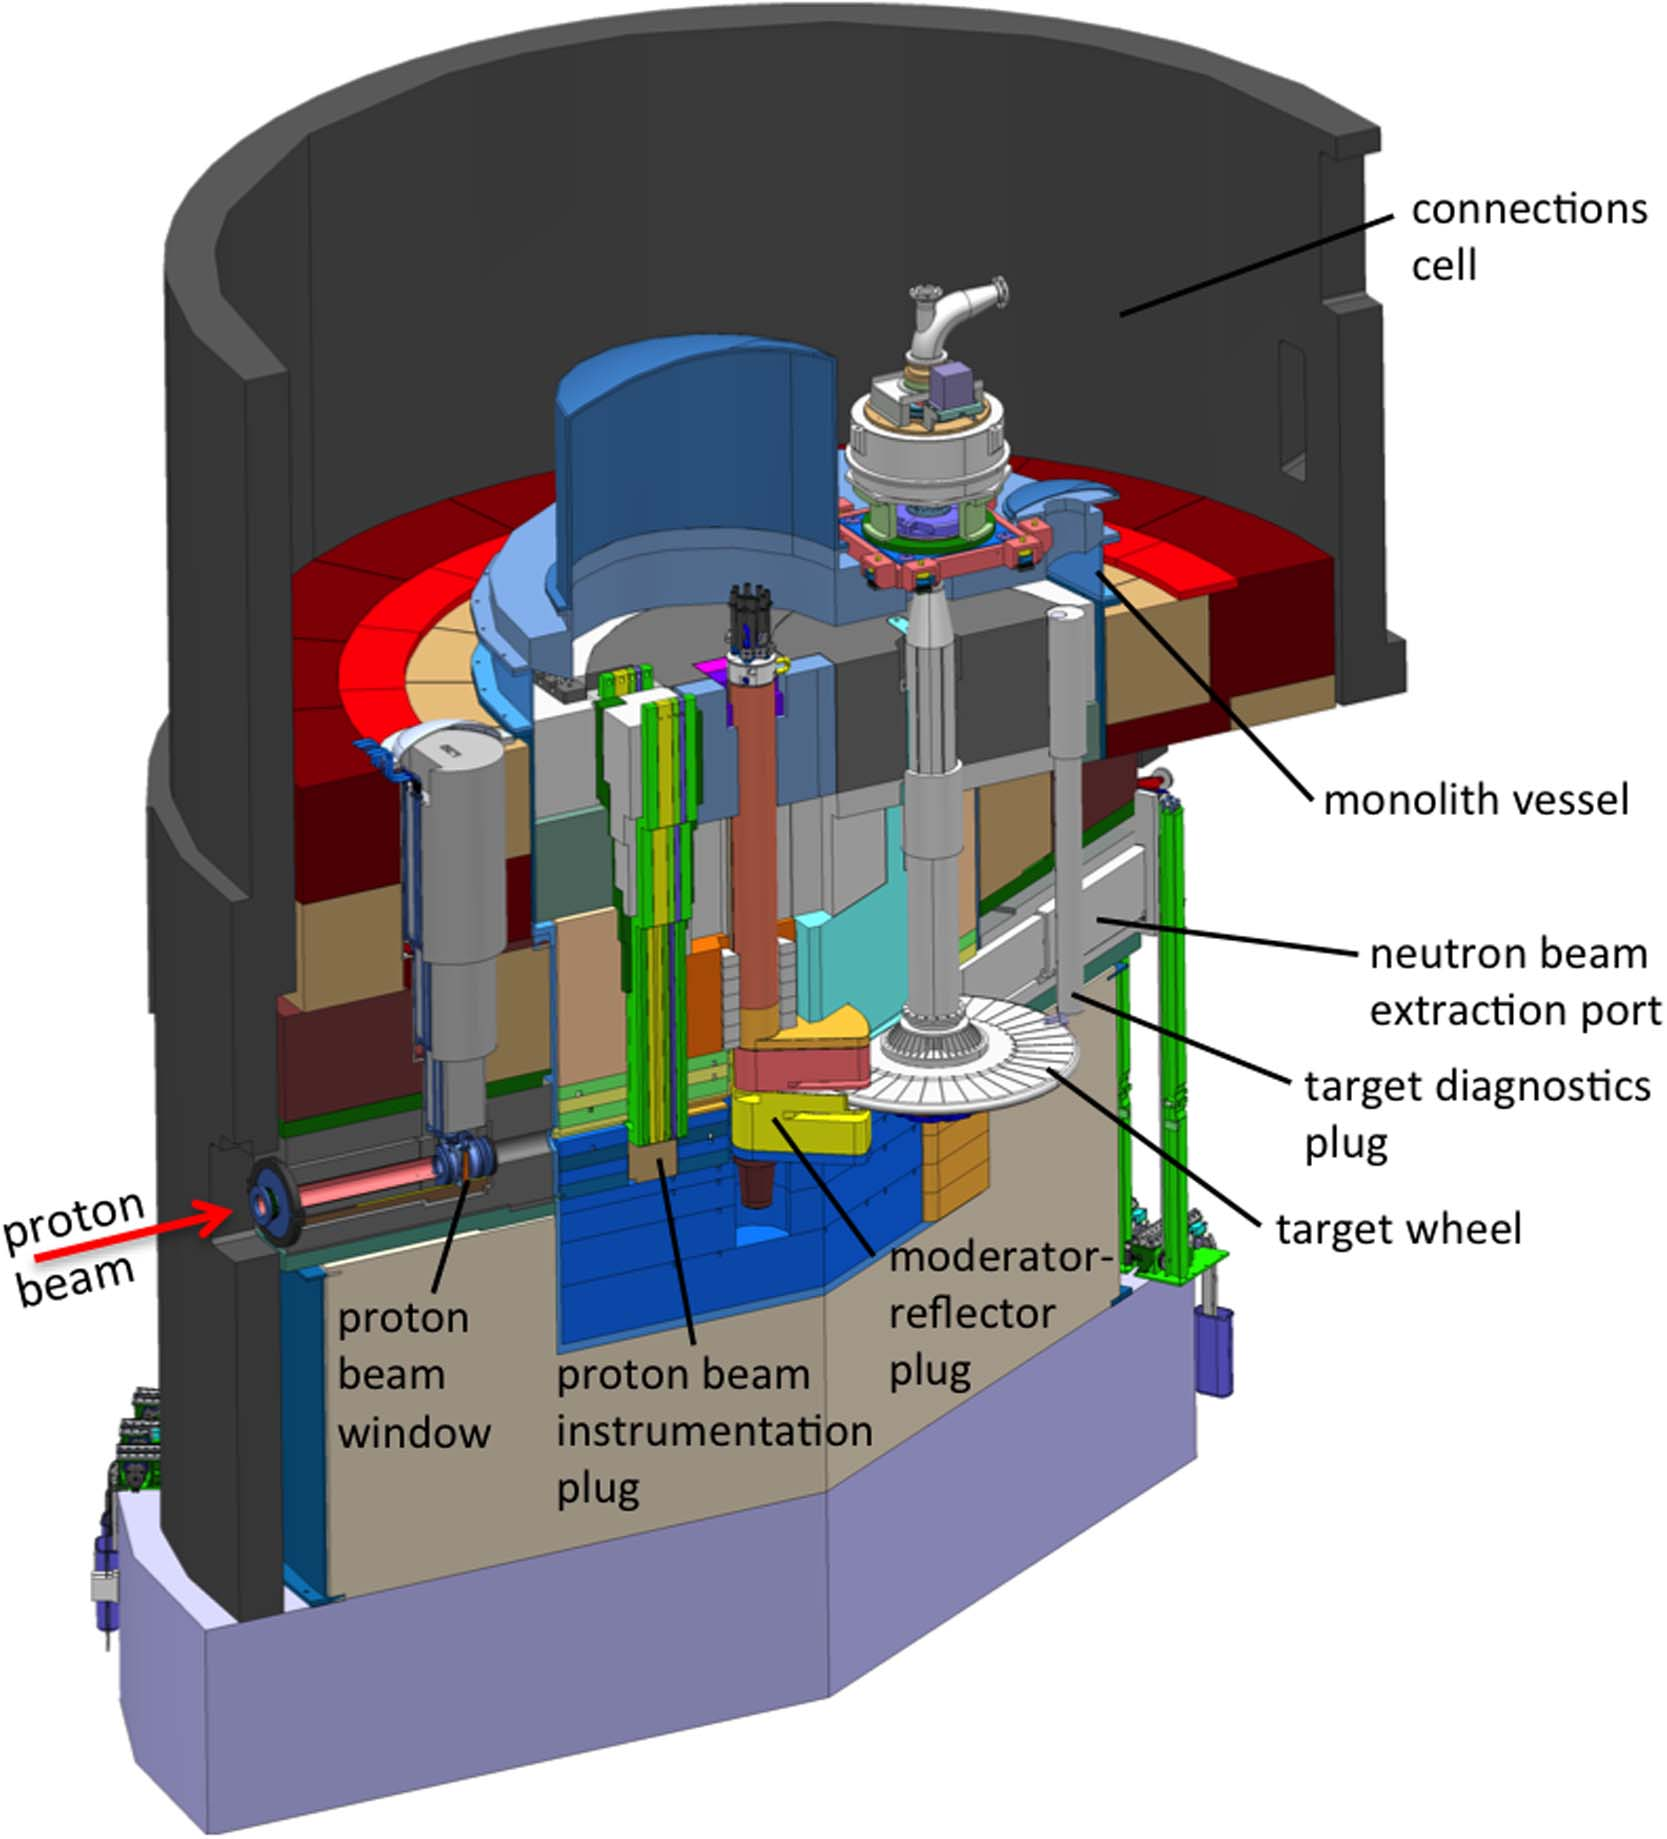
\includegraphics[width=\textwidth]{02_BeamDiag/figures/fig000_ESS_target_b}
	\end{center}
	\caption[The Tungsten target inside the monolith structure]{The Tungsten target inside the monolith structure.}
	\label{chap2:fig:target}
\end{figure}


  \section{ESS neutron instruments}

  When the \acrshort{ess} user programme will start in 2023, 15 instruments will be available for users. The installation of the first instruments began this year. These instruments have been reviewed and selected by scientific committees and validated by different \acrshort{ess} committees. Seven new instruments will be installed afterwards in a first extension phase. Finally in a more distant future, new instruments may be installed on the remaining neutron beam ports. Fig. \ref{chap3:fig:ESS_instruments} shows the setup of the 15 first neutron lines and instruments foreseen for the beginning of the user program. To give an idea of the scale, in the T-REX spectrometer the distance between the sample and the tungsten target is almost 170 meters.

  Each instrument is the result of close collaborations between \acrshort{ess} and numerous institutes specialized in neutron scattering. As already explained, \acrshort{ess} is a user facility and is open to both researchers and industrial actors from various fields. The different neutron scattering instruments at \acrshort{ess} will be used for a variety of applications. Therefore each instrument will be unique and will have to meet specific requirements. Table \ref{chap2:tab:ess_instruments} briefly summarizes the 15 initial instruments with some examples of areas of applications \cite{essInstrument,essInstrument2}.

  \begin{table}[ht]
  \centering
  \caption[Overview of ESS neutron instruments]
  {Overview of ESS neutron instruments \cite{essInstrument,essInstrument2}.}
  \label{chap2:tab:ess_instruments}
  \begin{tabularx}{\linewidth}{lXp{128pt}}
    \toprule
    Instrument & Description                              & Examples of application                                \\
    \midrule

    \multicolumn{3}{c}{Diffraction}                                                                                \\
    \midrule

    DREAM      & Bispectral powder diffractometer         & Crystallography, nanoscience, energy research          \\
    HEIMDAL    & Hybrid diffractometer                    & Magnetic properties, engineering                       \\
    MAGiC      & Magnetism single crystal diffractometer  & Magnetic properties                                    \\
    NMX        & Macromolecular crystallography           & Structural biology, drugs                              \\
    BEAR       & ToF diffractometer                       & Engineering                                            \\
    ODIN       & Multi-purpose neutron imaging instrument & Engineering, geo-science, paleontology                 \\

    \midrule

    \multicolumn{3}{c}{Reflectometry}                                                                              \\
    \midrule
    FREIA      & Liquids reflectometer                    & Life science, soft matter                              \\
    ESTIA      & Focusing reflectometer                   & Magnetic properties, thin films                        \\

    \midrule

    \multicolumn{3}{c}{SANS}                                                                                       \\
    \midrule
    LOKI       & Broadband SANS                           & Soft matter, biophysics                                \\
    SKADI      & General purpose SANS                     & Medical research, energy storage                                                      \\

    \midrule

    \multicolumn{3}{c}{Spectrometry}                                                                               \\
    \midrule
    T-REX      & Bisprectral chopper spectrometer         & Crystals, superconductivity                            \\
    VESPA      & Vibrational spectrometer                 & Chemistry, materials science                           \\
    MIRACLES   & Backscattering spectrometer              & Polymer science, energy materials, magnetic properties \\
    BIFROST    & Extreme environment spectrometer         & Engineering, superconductivity                         \\
    CSPEC      & Cold chopper spectrometer                & Life sciences,  materials, chemistry                   \\

    \bottomrule
  \end{tabularx}
\end{table}

  \vspace{1cm}

  \begin{figure}[!ht]
  \begin{center}
    \begin{subfigure}[t]{0.45\textwidth}
      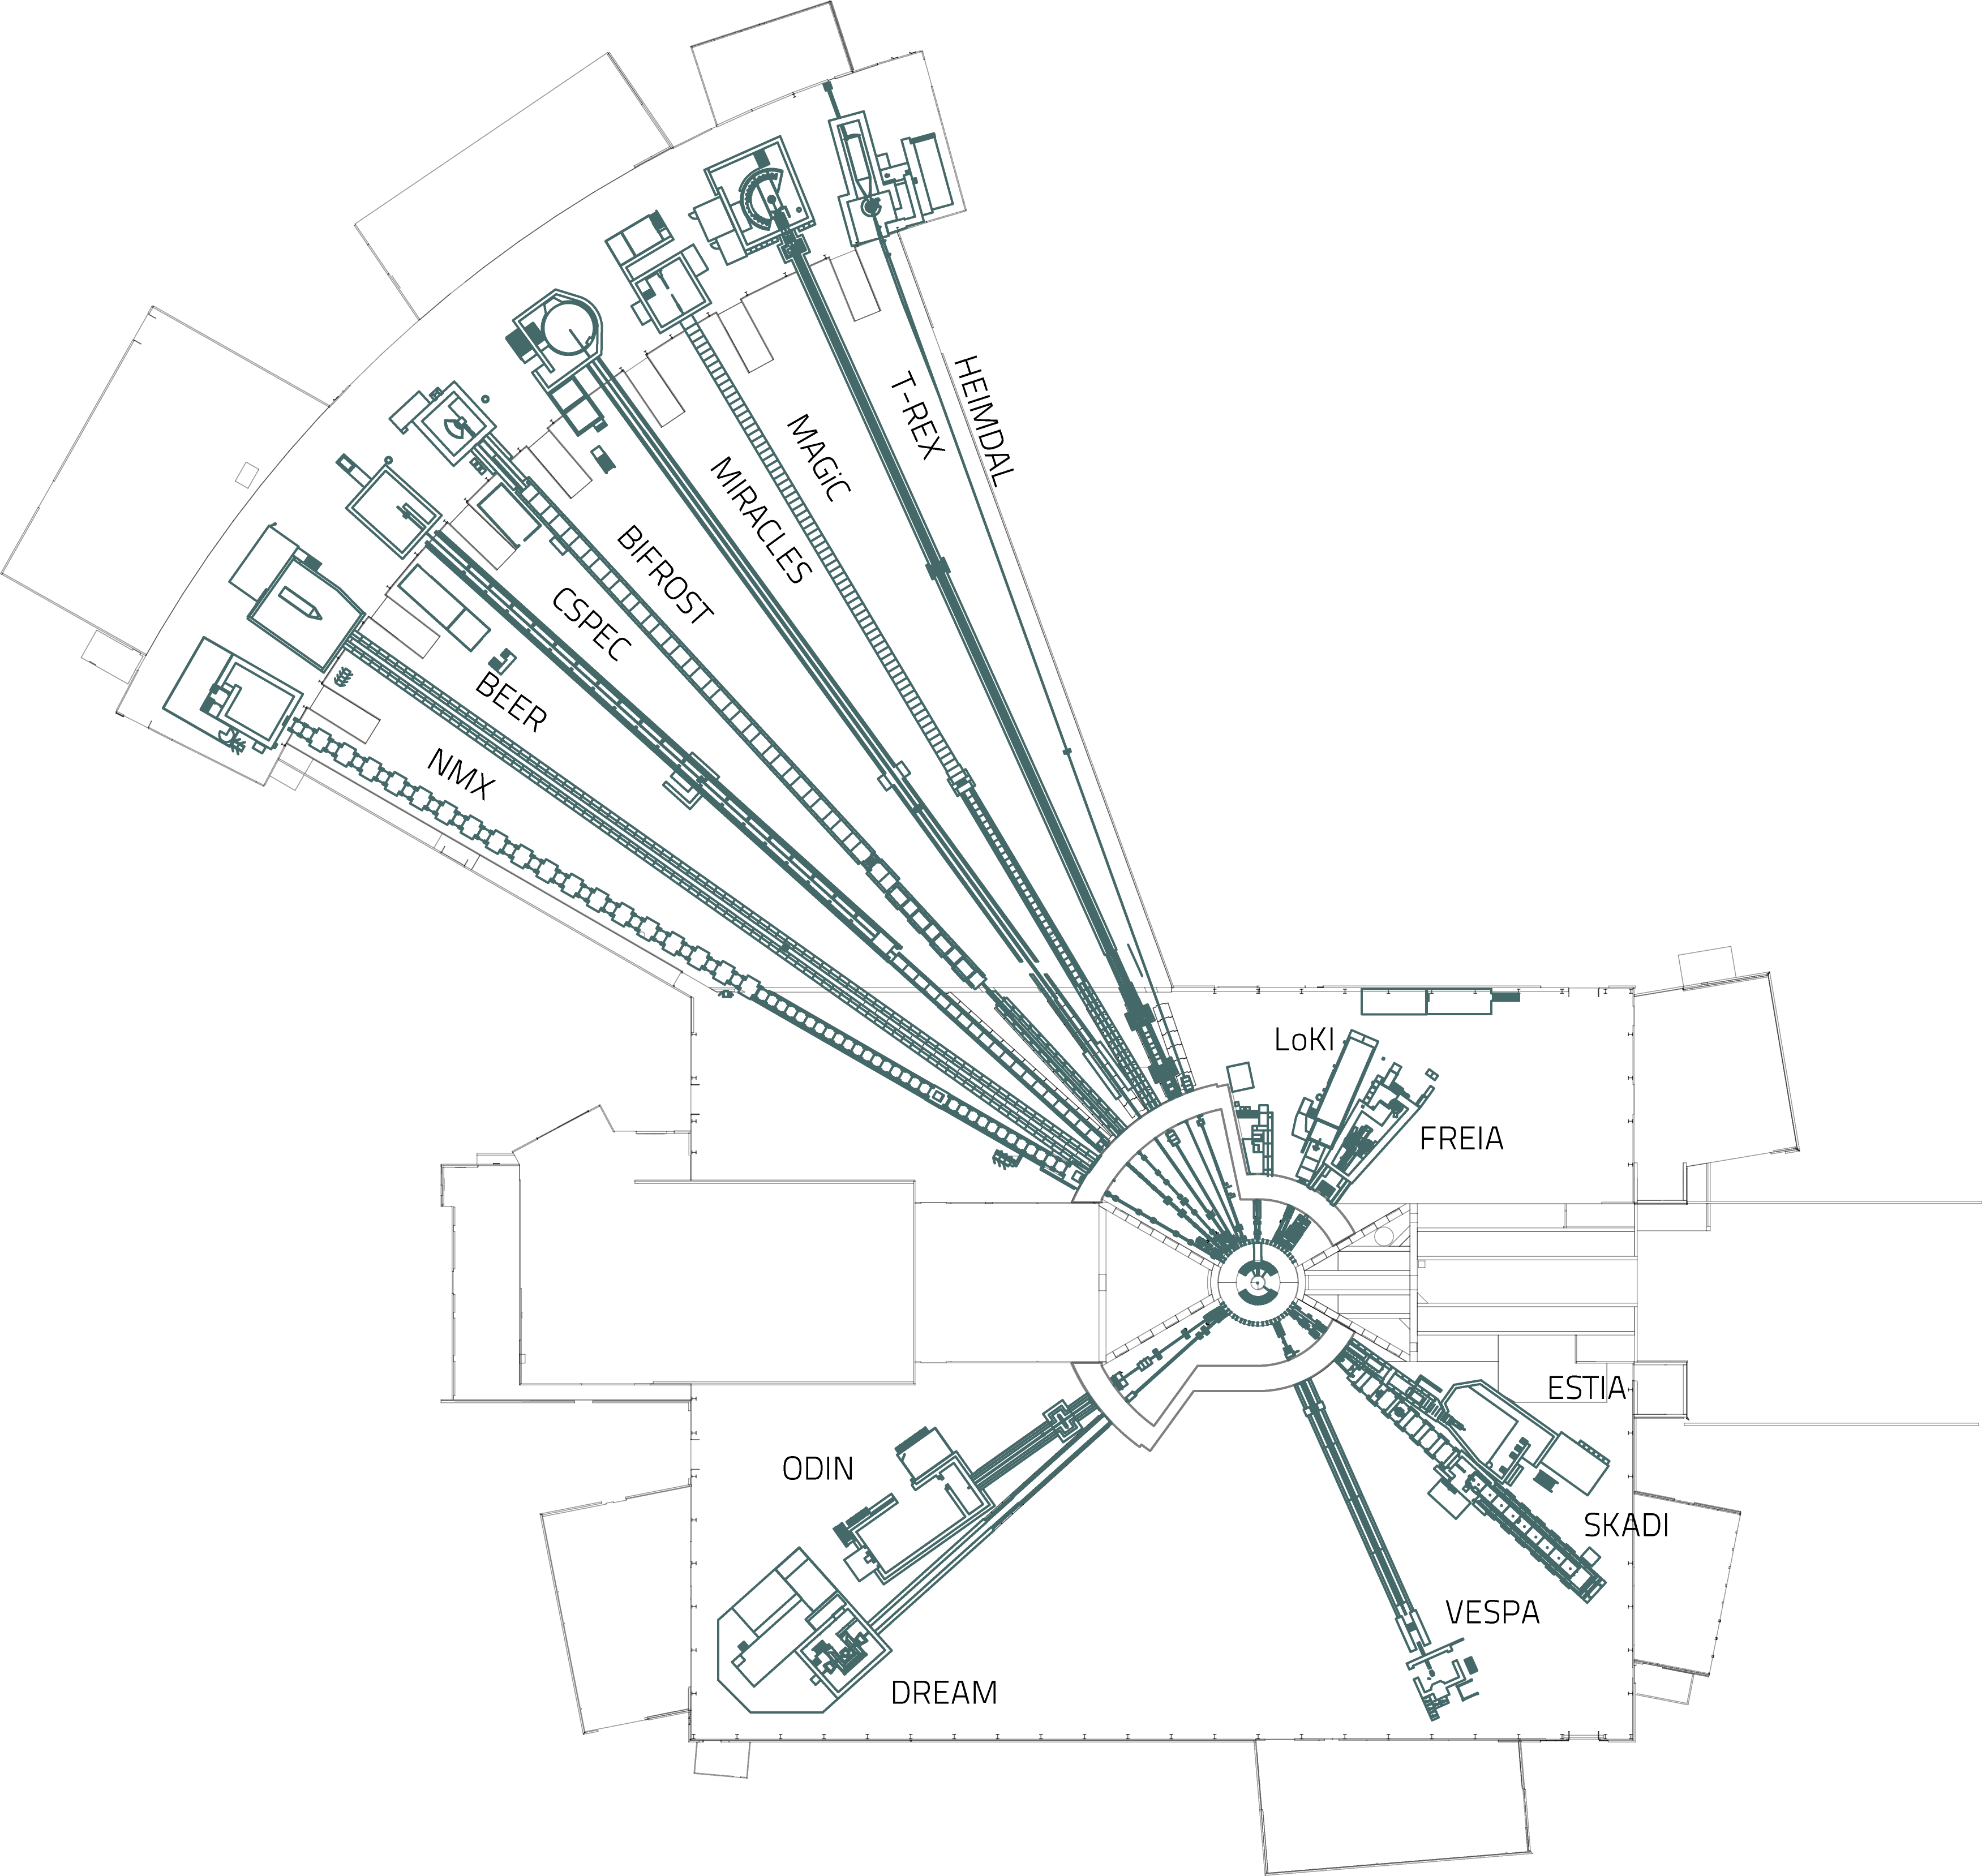
\includegraphics[width=\textwidth]{02_BeamDiag/figures/fig000_ESS_instruments}
      \caption{}
      \label{}
    \end{subfigure}
  \end{center}
  \caption[]{}
  \label{chap3:fig:ESS_instruments}
\end{figure}


  \FloatBarrier
  \section{Beam diagnostic overview}
  Beam diagnostics are used to ensure the proper functioning of the accelerator, as well as the safety of people and of the installation. They allow to measure the different beam characteristics such as current, position, beam losses, energy, profile, emittance etc. For each beam characteristic, several methods can be considered, each of them having advantages and drawbacks. Beam diagnostics are at the crossroads of many areas of physics and electronics, belonging to the so-call transverse activities.

  The accelerating technologies are often complicated and quite expensive. In general, the size of the accelerator is reduced as much as possible, the space along the beam tube is often limited. The choice of diagnostics installed on a line must therefore be done carefully according to the expectations. Neglecting diagnostics may be dramatic.

  The present section briefly\footnote{The CERN Accelerator School proceedings  dedicated to beam diagnostics is about 600 pages.} introduces different beam diagnostics frequently encountered on high intensity linear accelerators. Complete description of beam diagnostics can be found in books \cite{strehl2006}, Joint Universities Accelerator School \cite{juas2019} or CERN Accelerator School \cite{cas2019}.

  \subsection{Beam current monitor}
  % TODO: Référence
  The measurement of the beam current is perhaps the most basic information for an accelerator. Beam Current Monitors (\acrshort{bcm}) detect how many beam particle per time are passing through a specific position in the accelerator. The transmission between the different accelerating blocks can thus be quantified.

  The \acrshort{bcm}s rely on very different methods depending on the minimum value of the currents that should be achieved. For \acrshort{ess}, the beam current can be considered as high. Two common families of methods for measuring high currents are presented in this section.

  A \acrfull{fc} is a destructive method of current measurement. It can be seen as a beam dump, isolated from the accelerator ground, where the charges from the beam are collected by mean of a readout electronics. \acrshort{fc}s are often used in low energy parts of an accelerator (in the \acrshort{lebt} for instance) because they can operate both as current meters and beam dumps. At high energy, the size and the complexity of the \acrshort{fc} design considerably increase. A \acrshort{fc} is usually inserted downstream the iris allowing a fine current tuning, for avoiding the injection of the beam into the entire accelerator. The critical part of the \acrshort{fc} design is the cooling system that must be sufficiently efficient to dissipate the thermal power deposited by the beam. Repellers, like electrodes or permanent magnets, must be used to avoid any parasitic current due to secondary electron emissions, during the impact of the beam particles.

  A beam consists of many charged particles moving together within bunches, more or less in the same direction; therefore a beam generates an electromagnetic field. The magnetic field can be used to measure the beam current in a completely non-invasive manner by means of a current transformer (\acrshort{ct}). The beam can be seen as a one turn primary winding, and therefore the induced voltage measured on the secondary winding is proportional to the beam current (Fig. \ref{chap2:fig:CT}). 
  \begin{figure}[!ht]
	\begin{center}
		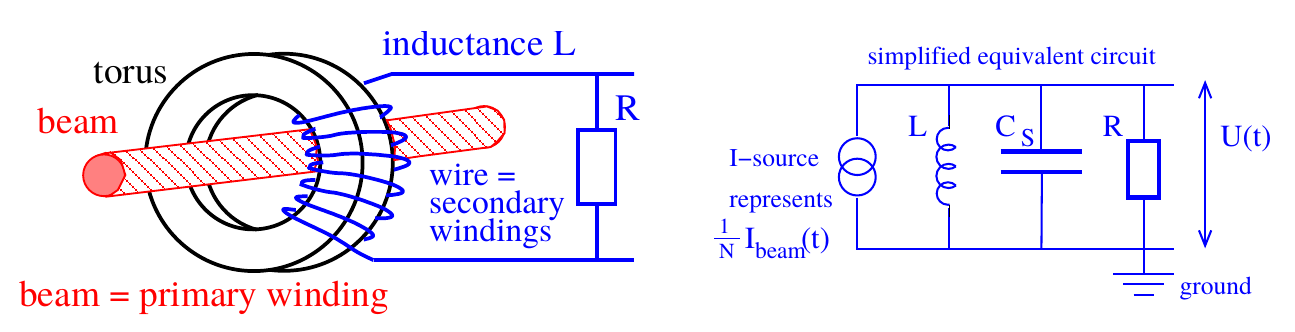
\includegraphics[width=\textwidth]{02_BeamDiag/figures/fig000_CT}
	\end{center}
	\caption[A simplified schema of a passive current transformer]{A simplified scheme of a passive current transformer \cite{ForkJUAS}.}
	\label{chap2:fig:CT}
\end{figure}

  
  The measurement in the secondary winding is carried out by an active device, an operational amplifier for instance, reducing the limitations of a passive measurement. Different implementations of current transformers exist depending on the requirements:
  \begin{itemize}
    \item Alternative Current Current Transformer (\acrshort{acct}): is the most common active transformer for pulsed beam.
    \item Fast Current Transformer (\acrshort{fct}): whose design is optimized for high-frequency current measurements, allowing bunch beam measurements for instance.
    \item Direct Current Current Transformer (\acrshort{dcct}): this type of transformers were developed to measure the DC component \cite{Unser1969} of a beam using a method similar to fluxgate sensor.
  \end{itemize}

  These diagnostics can be developed in-house or purchased directly off the shelf. At \acrshort{ess} \cite{Hassanzadegan:IPAC2018-WEPAF088}, 18 ACCTs from Bergoz Instrumentation \cite{bergoz2019} will be installed along the accelerator to measure the current. % \footnote{2 FCT are used in the MEBT}

  \subsection{Beam position monitor}
  The position measurement is also essential information to ensure the minimum operation of the accelerator. As explained in the previous section, the charged particles generate an electromagnetic field, and the electric field creates image charges on the vacuum walls \cite{strehl2006}. The distribution of these image charges depends, among other things, on the position of the beam in the vacuum chamber. These charges can be measured by setting an electrode, isolated from the walls, with a readout electronics. This type of detector is called a pick up monitor and is widely used for beam position measurement. In reality there are several types of pick up monitors whose operating principle are different and can not be covered here.

  % TODO: Few or some
  \begin{wrapfigure}{l}{0.35\textwidth}
  \centering
  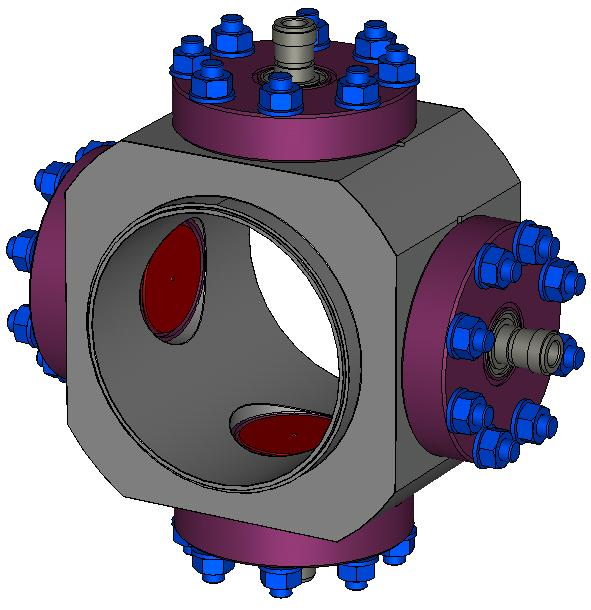
\includegraphics[width=0.35\textwidth]{02_BeamDiag/figures/fig000_BPM_button}
	\caption[A 3d drawing of the ESS button BPMs designed at DESY]{A 3d drawing of the ESS button BPMs designed at DESY.}
	\label{chap2:fig:BPM_button}
\end{wrapfigure}

  A button \acrshort{bpm} consists of four electrically isolated electrodes (buttons, visible in red on Fig. \ref{chap2:fig:BPM_button}), generally face to face, each button connected to a $50\,\Omega$ connector. The voltage due to the coupling between the beam and the button is then measured, and the position is calculated from the contributions of the four buttons. The measurement is not linear, so the value is corrected with a calibration factor, determined beforehand using a moving wire fed with \acrshort{rf} signal. The bandwidth of this type of \acrshort{bpm} is determined by the capacitance of the system (electrode, connection, cables), typically between $100\,\mathrm{MHz}$ and few GHz. Nowadays, the processing of the data relies on complex numerical \acrshort{rf} processing (filter, modulation, cordic decomposition). At \acrshort{ess}, the \acrshort{bpm} systems will be based on more than 90 \acrshort{bpm}s installed along the linac, mainly button-type \acrshort{bpm}s and few striplines.

  \subsection{Beam loss monitor}
  Beam Loss Monitors (\acrshort{blm}) are mandatory diagnostics in all accelerators, mainly in high power accelerator facilities. When particles are lost in the accelerator, they hit and pass through the beam tube elements producing different type of radiation. In an accelerator, the primary goal of \acrshort{blm} systems is to guarantee the safety of the installation. Indeed, when the loss rates are high, the devices around the accelerator can be severely damaged.

  \acrshort{blm}s are very often connected to the machine protection system (\acrshort{mps}) allowing a fast shut down of the accelerator if the losses are too high. \acrshort{blm}s relies on a wide range of radiation detection techniques.

  At \acrshort{ess} two types of \acrshort{blm} are foreseen. The first type of beam loss monitors is based on ionization chambers (\acrshort{icblm}) \cite{Grishin:IBIC2017-WEPWC03}. These are the most common \acrshort{blm} types; \acrshort{icblm}s are widely used at CERN in \acrshort{lhc} \cite{HOLZER20122055}, \acrshort{sns} etc. In an \acrshort{icblm}, the losses ionize the gas in the chamber and a current is established between the electrodes. An \acrshort{icblm} has a high dynamic range, fast response and is cost effective.

  \begin{figure}[!ht]
	\begin{center}
		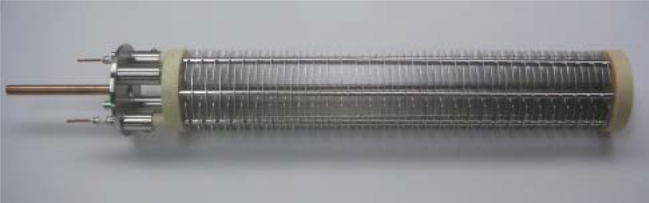
\includegraphics[width=\textwidth]{02_BeamDiag/figures/fig000_icBLM}
	\end{center}
	\caption[The ionization chamber of an icBLM]{The ionization chamber of an icBLM.}
	\label{chap2:fig:icBLM}
\end{figure}


  The second type of \acrshort{ess} \acrshort{blm}s is completely new: the neutron Beam Loss Monitors (\acrshort{nblm}) \cite{Papaevangelou:HB2018-THA1WE04}.
  A acrshort{nblm} is sensitive to fast neutrons and insensitive to photons ($X$ and $\gamma$) emitted by the accelerator cavities. In fact, two acrshort{nblm} types, based on Micromegas detectors \cite{GIOMATARIS199629} were developed:
  \begin{itemize}
    \item A fast detector ($<\,50\,\mathrm{ns}$), sensitive to high losses allowing a very fast stopping of the beam.
    \item A slower detector ($<\,200\,\mathrm{\mu s}$), with a higher sensitivity, allowing a finer monitoring of the losses.
  \end{itemize}

  A total of 266 \acrshort{icblm}s, 42 slow acrshort{nblm} and 42 fast acrshort{nblm} will be installed along the accelerator.

  %\subsection{Beam emittance measurements}

  \section{Invasive beam profile measurements}
  \subsection{Interceptive screen}
  A luminescent screen provides a convenient way to measure profiles since this diagnostic is simple to implement. The screen is inserted directly in the beam path using an actuator. When particles pass through the material, they partly deposit their energies, exciting the medium. During the de-excitation process, most of the energy is released under the form of visible photons. The intensity of light from the screen is proportional to the number of incident particles and their energy deposition. It is possible to measure, with a single camera, the beam profile in two dimensions simply by tilting the screen.

  The use of this diagnostic is strongly limited by the energy and intensity of the beam. At low energies and/or high current, the power to be dissipated can be locally considerable, reaching saturation and altering the screen properties. In general, a permanent decrease of the light yield is observed \cite{Simon:IBIC2016-MOPG79} and in some extreme cases a deterioration of the screen surface is remarked.

  A concrete use of this type of diagnostics will be briefly presented in Chapter 4 with some experimental results.

  There is another type of intrusive diagnostics based on the optical transition radiation. The setup looks similar to the one just described, but the process behind is totally different. When a relativistic particle is subject to a sudden variation of the dielectric constant, i.e. passes the border of two different media, transition photons are emitted with precise angles depending on the particle, its velocity and the angle of incidence. This method is well adapted for high relativistic accelerators such as $e^{-}$ \acrshort{linac} \cite{Nolle2009,Bolzon2013}.

  \subsection{Wire scanner}
  A Wire Scanner (\acrshort{ws}) is an invasive diagnostics that probes the beam with a micrometer wire, taut on a movable fork. The measurement in both directions of the transverse profile is possible by using a wire set at certain angle (typically 45°) with respect to the \acrshort{ws} translation. Two detection modes are possible depending on the energy of the beam to be analyzed.

  The secondary electron emission mode is adapted to low beam energies. When the beam passes through the wire, secondary electrons are emitted from the surface of the wire and the other electron-ion pairs are absorbed into the wire. The current read on the wire is proportional to the number of emitted electrons. As the beam deposits its energy, the wire also heats up; note that in a vacuum it is only cooled by radiation and conduction with the fork. At certain, temperature the wire starts to emit electrons by thermoionic effect. This effect is not linear and interferes with the measurement.

  For high energy beams, the detection strategy is completely different. When an energetic beam interact with the wire, electromagnetic cascades may occur. The shower can be detected outside the beam tube using a fast calorimeter. The most common calorimeter are scintillators.% which are sensitive, fast and easily couple with other devices like . 

  The design of the wire is usually done in two steps \cite{Cheymol:LINAC2014-MOPP036}. The number of emitted electrons and the deposited energy is calculated first, for instance with Monte Carlo codes. Then thermal simulations are performed, with numerical partial differential equation solver, to determine the heating that occurs in a wire during the pulses. The two most commonly used materials for wires are tungsten and carbon, which have respectively very high melting and sublimation temperatures. The diameter of the beam is optimized according to the simulations and the wire material, typical the diameter of a wire is between $20$ and $100\,\mathrm{\mu m}$.

  The method is sensitive to low beam currents. Wire scanners are used in linacs mainly in low current and/or at low cycle beam. In synchrotrons, the multiple passages of the beam leads to rapid heating of the wires.
  For both accelerators, the design of the wires is crucial. The interaction time must be minimized with fast translators. This is the flying wire method used on synchrotrons.

  At \acrshort{ess} both types of wire are used, 3 \acrshort{sem}-\acrshort{ws} will be installed in the \acrshort{mebt}. Then 10 electromagnetic-\acrshort{ws} will be installed in the superconducting part \cite{Cheymol:HB2016-MOPL018}. The wire scanners will be used mainly during the commissioning of the machine, in fact the wire can withstand the beam power only during low duty cycle ($100\,\mathrm{\mu s}$ at the nominal \acrshort{ess} current).

  \subsection{SEM-Grid}
  A Secondary Electron EMission grid (\acrshort{sem}-Grid) or harp grid is a multichannel version of the \acrshort{sem}-\acrshort{ws}. Several wires are taut on a frame in the same direction at several positions. To avoid crosstalk due to secondary electrons, an electron repeller (wire or electrode) is often set around the wires. A second wire plane can also be set in the transverse direction. Both grids are inserted in the beam tuned at low duty cycle and both profiles (X and Y) are measured in one shot. By using several \acrshort{sem}-grids successively the measurement of the transverse emittance is possible.

  However, the readout electronics of the secondary emission currents of all wires is more complex due to the number of channels. The number of wires must be chosen according to the resolution requirements on the beam sizes and positions. The wires must meet the same constraints as the wire scanner. The system is not necessarily more robust because if one wire breaks it may short-circuit the other wires nearby.

  \section{Non-invasive beam profile measurements}
  \subsection{Laser wire profiler}
  For negative ion beams, a specific method, based on photo neutralization process, allows an almost (considering beam particle losses that occur along the accelerator) non invasive profile measurement. Photo neutralization works as follows: when a photon has a sufficient energy, it can strip off an electron of a negative ion.
  The photo neutralization cross section depends mainly on the energy of ions and on the wavelength of photons. With a dipole magnet free electrons are separated from the $H^-$ beam. Then, the electrons are collected and detected by a Faraday cup, a \acrshort{mcp} or a semiconductor detector. The transverse profile is reconstructed by scanning the laser in the beam like a wire scanner.

  This kind of device is popular on $H^-$ ion accelerators such as \acrshort{sns} \cite{LIU2010241} and LINAC4 \cite{Hofmann2015}. The method does not require any element passing through the beam. Therefore the laser wire scanners are very well suited for high intensity beams. The method requires an advanced laser system (typically $1064\,\mathrm{nm}$ Nd:YAG laser in $\mathrm{mJ}$ range) \footnote{The laser can distributed on several measuring stations with optical fibers.} as well as quite complicated optical setups.

  \subsection{Fluorescence Profile Monitor}
  Fluorescence Profile Monitors (\acrshort{fpm}) or Beam Induced Fluorescence (\acrshort{bif}) monitors are non-invasive diagnostics for transverse profile measurements. When the particles of the beam pass through the residual gas, they can excite the residual gas. Fluorescence photons are emitted when the excited molecules return to their fundamental states.

  The fluorescence is a luminescent process characterized by a rapid de-excitation (few tens of nanoseconds). The fluorescence can occur with gases and each gas has its own emission spectra. Some gases have much larger effective cross-sections such as nitrogen, which is very often used. Fig. \ref{chap3:fig:FPM} shows a classic \acrshort{fpm} assembly with an amplified detection readout and a gas injection system. In an ideal case, the light reflection capability of the vacuum chamber, where a \acrshort{fpm} is mounted, must be as low as possible for reducing the background signal. This is commonly achieved by applying a black coating on the surface.

  \begin{wrapfigure}{r}{0.35\textwidth}
  \begin{center}
		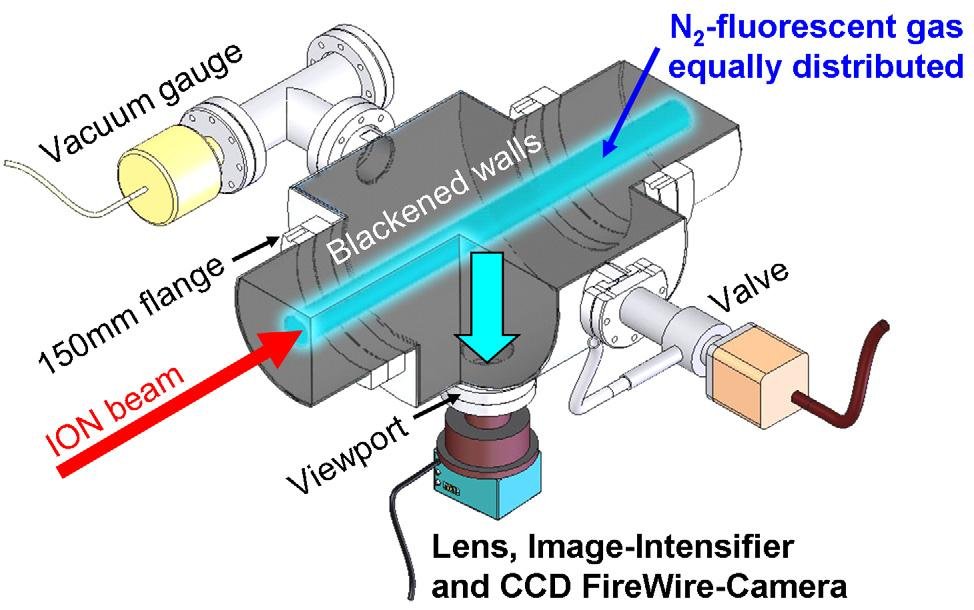
\includegraphics[width=0.35\textwidth]{02_BeamDiag/figures/fig000_FPM}
	\end{center}
	\caption[Scheme of a BIF setup used at GSI.]{Scheme of a BIF setup used at GSI \cite{ForckJUAS}.}
	\label{chap3:fig:FPM}
\end{wrapfigure}

  Light detection is however limited by several factors. The fluorescence photon is emitted within $4\pi$ steradians, so the signal collected depends on the solid angle subtended by the detector. The fluorescence cross section follows the Bloch equation and decreases very quickly with the energy. \acrshort{fpm}s are therefore preferred for low energy beam lines where the pressure is high. Otherwise, a \acrshort{fpm} requires a gas injection system to increase the signal.

  This kind of detector will be installed almost everywhere at \acrshort{ess} \cite{Thomas2016} except in the superconducting part where the very low pressure ($10^{-9}\,\mathrm{mbar}$) and high beam energy no longer allows profile measurements with \acrshort{fpm}s. Gas injection is not desired in the superconducting part of the accelerator.

  \section{Ionization Profile Monitor and summary}
  In the previous sections different methods for measuring the transverse profile have been presented. None of these methods may be able to measure the transverse profile in the superconducting part of \acrshort{ess} at nominal beam conditions. Wire scanners are very common devices but can not handle the beam power under the nominal conditions. Moreover if one single wire melts it could contaminate the surrounding cavities. Laser Wire scanners are very elegant solutions, but they can only work with negative ions. The very low pressures in the cryogenic part prevents the use of \acrshort{fpm}s and gas injection is not allowed at \acrshort{ess}.

  As the superconducting accelerating part of the \acrshort{ess} linac is the longest in terms of acceleration elements, it would be harmful to leave this entire section without any transverse profile diagnostics.

  A \acrfull{bgi} profile monitor or an \acrfull{ipm} is based on the direct collection of ionization by-products from the residual gas by an electric field. In the following we will use only the name \acrshort{ipm} and the operation will be explained in much more detail in the next chapter. The method is non invasive as long as the electrical field does not bend the beam too much. An \acrshort{ipm} is more complicated to implement and requires to set up some systems in vacuum. \acrshort{ipm}s are quite common diagnostics on proton and hadron storage rings where pressures are very low, but they became popular on linear accelerators with the increasing use of superconducting cavities.

  The method has been known since the late 1960s, but is continuously evolving with technological progress. First in terms of computing: nowadays computers are able to solve electromagnetic field equations, which greatly improves the understanding of \acrshort{ipm}s making possible to figure out and correct various errors on measurements. Moreover, the electronics become more and more sensitive, precise and fast. In the 90s, the rise of particle amplifiers, like MicroChannel Plates and Channeltrons, have permitted the \acrshort{ipm}s to operate under even more critical conditions in terms of energy and vacuum.
  Recently, the interest in semiconductor detectors has grown and an innovative \acrshort{ipm} project using TimePix3 detectors is under development at \acrshort{cern} for the \acrshort{ps} \cite{Storey2015}. The first results are very promising \cite{Storey2017} and offer a new perspective on \acrshort{ipm} usages.

  The \acrshort{ipm} method is now mature and used in several installations \cite{Krider1989,Wittenburg1992,Satou2006,Giacomini2011,Morris2011,egberts2012}.
  Fig. \ref{chap2:fig:IPM_3} shows 3 \acrshort{ipm}s installed on 3 different accelerators. One can see directly that the design of an \acrshort{ipm} is unique and tailor-made for its accelerator. This thesis deals with the development of \acrshort{ipm}s for the superconducting part of the \acrshort{ess} accelerator. The different \acrshort{ipm} technologies have been reviewed in order to select the most efficient one with respect to the \acrshort{ess} requirements.

  \begin{figure}[!ht]
  \centering
  \begin{subfigure}[t]{0.45\textwidth}
    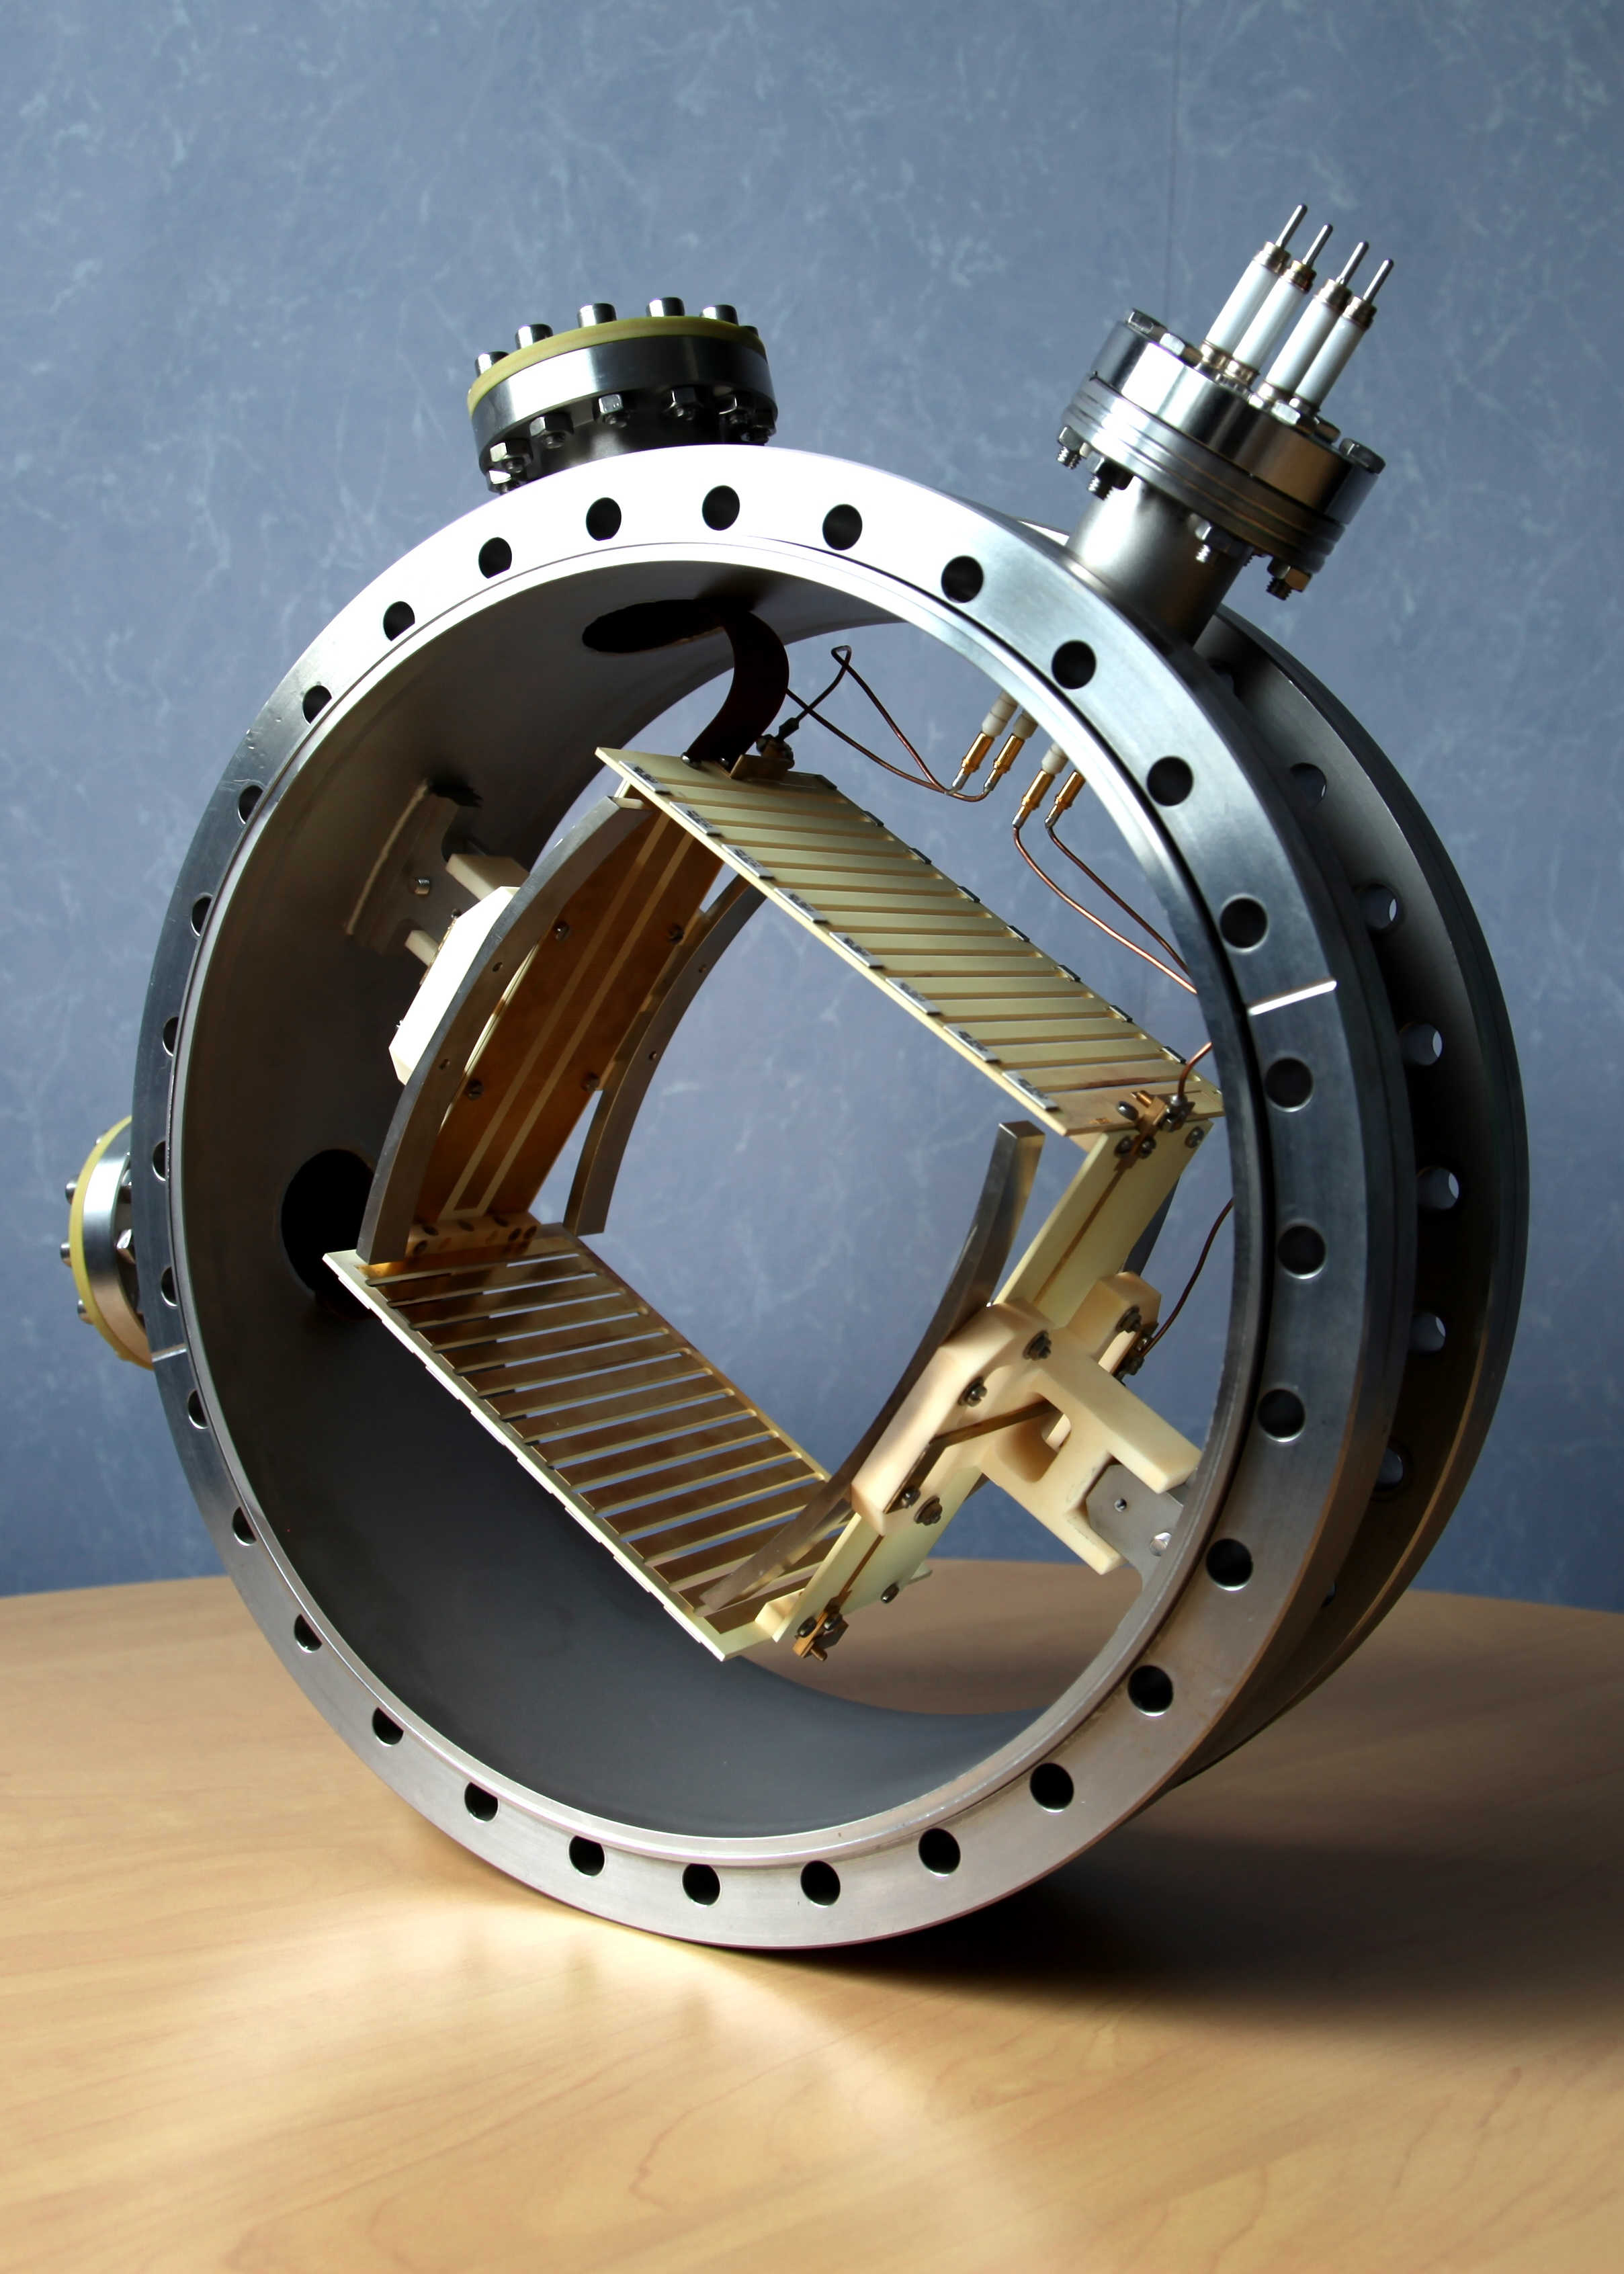
\includegraphics[width=\textwidth]{02_BeamDiag/figures/fig000_IPM_1}
    \caption[One of the IPM at IFMIF]{One of the IPM at IFMIF \cite{egberts2012}.}
    \label{}
  \end{subfigure}
  ~
  \begin{subfigure}[t]{0.45\textwidth}
    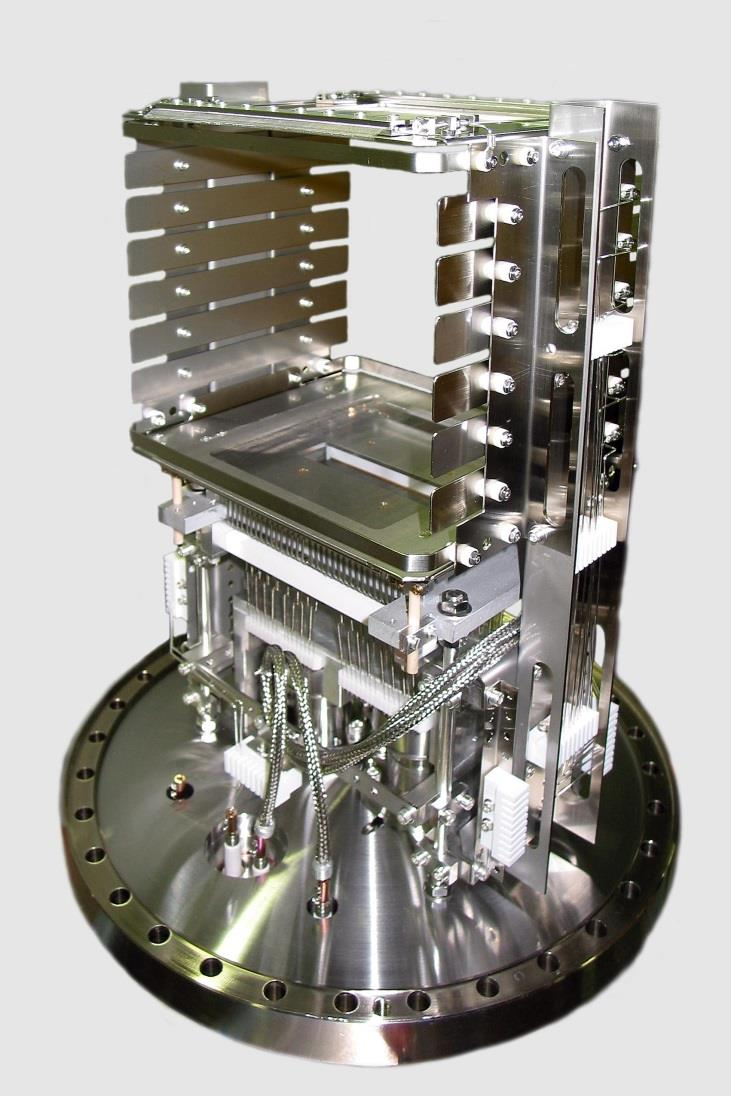
\includegraphics[width=\textwidth]{02_BeamDiag/figures/fig000_IPM_2}
    \caption[One of the IPM at GSI]{One of the IPM at GSI \cite{ForkJUAS}.}
    \label{}
  \end{subfigure}
  
  \begin{subfigure}[t]{1\textwidth}
    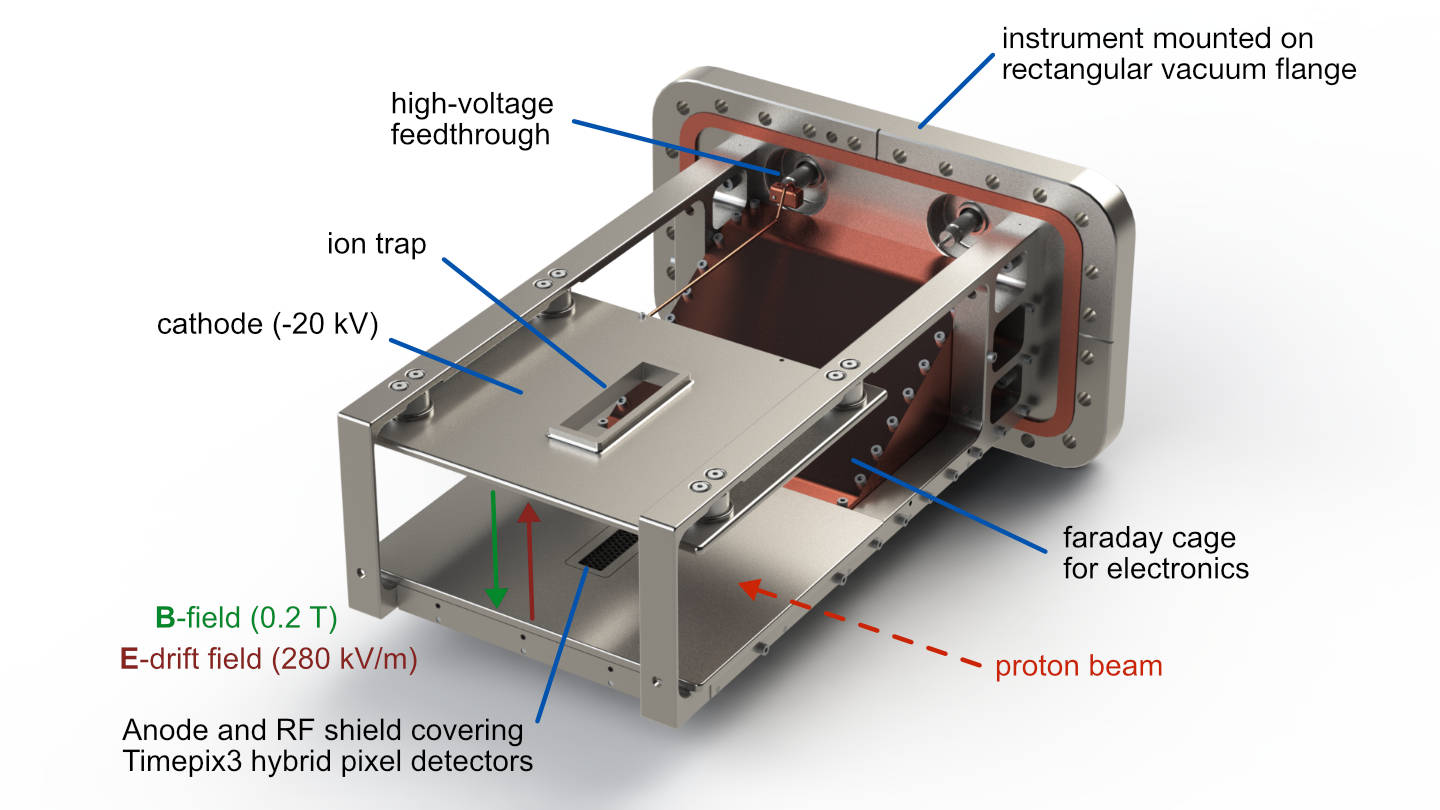
\includegraphics[width=\textwidth]{02_BeamDiag/figures/fig000_IPM_3}
    \caption[The future IPM for the PS]{The future IPM for the PS \cite{Storey2017}.}
    \label{}
  \end{subfigure}
  \caption[Three different implementations of IPMs on three different accelerators]{Three different implementations of IPMs on three different accelerators.}
  \label{chap2:fig:IPM_3}
\end{figure}


  \cleardoublepage
  \section*{Bibliography}
  \addcontentsline{toc}{section}{Bibliography}
  \label{ch2:bib}
  \printbibliography[heading=subbibliography]

\end{refsection}
